%%%%%%%%%%%%%%%%%%%%%%%%%%%%%%%%%%%%%%%%%
% Masters/Doctoral Thesis 
% LaTeX Template
% Version 2.5 (27/8/17)
%
% This template was downloaded from:
% http://www.LaTeXTemplates.com
%
% Version 2.x major modifications by:
% Vel (vel@latextemplates.com)
%
% This template is based on a template by:
% Steve Gunn (http://users.ecs.soton.ac.uk/srg/softwaretools/document/templates/)
% Sunil Patel (http://www.sunilpatel.co.uk/thesis-template/)
%
% Template license:
% CC BY-NC-SA 3.0 (http://creativecommons.org/licenses/by-nc-sa/3.0/)
%
%%%%%%%%%%%%%%%%%%%%%%%%%%%%%%%%%%%%%%%%%

%----------------------------------------------------------------------------------------
%	PACKAGES AND OTHER DOCUMENT CONFIGURATIONS
%----------------------------------------------------------------------------------------

\documentclass[
12pt, % The default document font size, options: 10pt, 11pt, 12pt
oneside, % Two side (alternating margins) for binding by default, uncomment to switch to one side
english, % ngerman for German
doublespacing, % Single line spacing, alternatives: singlespacing or onehalfspacing
%draft, % Uncomment to enable draft mode (no pictures, no links, overfull hboxes indicated)
%nolistspacing, % If the document is onehalfspacing or doublespacing, uncomment this to set spacing in lists to single
%liststotoc, % Uncomment to add the list of figures/tables/etc to the table of contents
%toctotoc, % Uncomment to add the main table of contents to the table of contents
parskip, % Uncomment to add space between paragraphs
%nohyperref, % Uncomment to not load the hyperref package
headsepline, % Uncomment to get a line under the header
chapterinoneline, % Uncomment to place the chapter title next to the number on one line
%consistentlayout, % Uncomment to change the layout of the declaration, abstract and acknowledgements pages to match the default layout
]{MastersDoctoralThesis} % The class file specifying the document structure

\usepackage{lmodern} % for bold teletype font
\usepackage{minted}
\usepackage{amsmath}
\usepackage{float}
\usepackage{subcaption}
\usepackage{amsmath}

\usepackage[utf8]{inputenc} % Required for inputting international characters
\usepackage[T1]{fontenc} % Output font encoding for international characters

\usepackage{mathpazo} % Use the Palatino font by default

\usepackage[backend=bibtex,style=numeric,natbib=true]{biblatex} % Use the bibtex backend with the authoryear citation style (which resembles APA)

\addbibresource{example.bib} % The filename of the bibliography

\usepackage[autostyle=true]{csquotes} % Required to generate language-dependent quotes in the bibliography

%----------------------------------------------------------------------------------------
%	MARGIN SETTINGS
%----------------------------------------------------------------------------------------

\geometry{
	paper=a4paper, % Change to letterpaper for US letter
	inner=2.5cm, % Inner margin
	outer=3.8cm, % Outer margin
	bindingoffset=.5cm, % Binding offset
	top=1.5cm, % Top margin
	bottom=1.5cm, % Bottom margin
	%showframe, % Uncomment to show how the type block is set on the page
}

%----------------------------------------------------------------------------------------
%	THESIS INFORMATION
%----------------------------------------------------------------------------------------

\thesistitle{Finite Difference Time Domain Method Implementation in C++} % Your thesis title, this is used in the title and abstract, print it elsewhere with \ttitle
\supervisor{Prof. Dr. Peter  \textsc{Thoma}} % Your supervisor's name, this is used in the title page, print it elsewhere with \supname
\examiner{Prof. Dr. Egbert \textsc{Falkenberg}} % Your examiner's name, this is not currently used anywhere in the template, print it elsewhere with \examname
\degree{Master of Science} % Your degree name, this is used in the title page and abstract, print it elsewhere with \degreename
\author{Xhoni \textsc{Robo}} % Your name, this is used in the title page and abstract, print it elsewhere with \authorname
\addresses{} % Your address, this is not currently used anywhere in the template, print it elsewhere with \addressname

\subject{} % Your subject area, this is not currently used anywhere in the template, print it elsewhere with \subjectname
\keywords{Finite, Time, Domain, Difference, C++, High, Integrity, Systems, 1D, 2D, 3D} % Keywords for your thesis, this is not currently used anywhere in the template, print it elsewhere with \keywordnames
\university{\href{https://www.frankfurt-university.de/}{Frankfurt University of Applied Sciences}} % Your university's name and URL, this is used in the title page and abstract, print it elsewhere with \univname
\department{} % Your department's name and URL, this is used in the title page and abstract, print it elsewhere with \deptname
\group{High Integrity Systems} % Your research group's name and URL, this is used in the title page, print it elsewhere with \groupname
\faculty{\href{https://www.frankfurt-university.de/de/hochschule/fachbereich-2-informatik-und-ingenieurwissenschaften/willkommen-am-fb-2/}{Faculty 2: Computer Science and Engineering}} % Your faculty's name and URL, this is used in the title page and abstract, print it elsewhere with \facname

\AtBeginDocument{
\hypersetup{pdftitle=\ttitle} % Set the PDF's title to your title
\hypersetup{pdfauthor=\authorname} % Set the PDF's author to your name
\hypersetup{pdfkeywords=\keywordnames} % Set the PDF's keywords to your keywords
}

\begin{document}

\frontmatter % Use roman page numbering style (i, ii, iii, iv...) for the pre-content pages

\pagestyle{plain} % Default to the plain heading style until the thesis style is called for the body content

%----------------------------------------------------------------------------------------
%	TITLE PAGE
%----------------------------------------------------------------------------------------

\begin{titlepage}
\begin{center}

{\scshape\LARGE \univname\par}\vspace{1.5cm} % University name
\textsc{\Large Master Thesis}\\[0.5cm] % Thesis type

\HRule \\ % Horizontal line
{\huge \bfseries \ttitle\par}\vspace{0.4cm} % Thesis title
\HRule \\ % Horizontal line
 
\begin{minipage}[t]{0.4\textwidth}
\begin{flushleft} \large
\emph{Author:}\\
{\authorname} % Author name - remove the \href bracket to remove the link
\end{flushleft}
\end{minipage}
\begin{minipage}[t]{0.4\textwidth}
\begin{flushright} \large
\emph{Supervisor:} \\
{\supname} \\ % Supervisor name - remove the \href bracket to remove the link
\emph{Assistant Supervisor:} \\
{\examname} % Examiner name - remove the \href bracket to remove the link  
\end{flushright}
\end{minipage}\\[1.0cm]


\large \textit{A thesis submitted in fulfillment of the requirements\\ for the degree of \degreename}\\[0.3cm] % University requirement text
\textit{in}\\[0.4cm]
\groupname\\\facname\\[0.5cm] % Research group name and department name
 
\vfill

{\large \today}\\[2cm] % Date
%\includegraphics{Logo} % University/department logo - uncomment to place it
 
\vfill
\end{center}
\end{titlepage}

%----------------------------------------------------------------------------------------
%	DECLARATION PAGE
%----------------------------------------------------------------------------------------

\begin{declaration}
\addchaptertocentry{\authorshipname} % Add the declaration to the table of contents
\noindent I, \authorname, declare that this thesis titled, \enquote{\ttitle} and the work presented in it are my own. I confirm that:

\begin{itemize} 
\item This work was done wholly or mainly while in candidature for a research degree at this University.
\item Where any part of this thesis has previously been submitted for a degree or any other qualification at this University or any other institution, this has been clearly stated.
\item Where I have consulted the published work of others, this is always clearly attributed.
\item Where I have quoted from the work of others, the source is always given. With the exception of such quotations, this thesis is entirely my own work.
\item I have acknowledged all main sources of help.
\item Where the thesis is based on work done by myself jointly with others, I have made clear exactly what was done by others and what I have contributed myself.\\
\end{itemize}
 
\noindent Signed:\\
\rule[0.5em]{25em}{0.5pt} % This prints a line for the signature
 
\noindent Date:\\
\rule[0.5em]{25em}{0.5pt} % This prints a line to write the date
\end{declaration}

%----------------------------------------------------------------------------------------
%	ABSTRACT PAGE
%----------------------------------------------------------------------------------------

\begin{abstract}
\addchaptertocentry{\abstractname} % Add the abstract to the table of contents
This thesis is the final documentation for a project in the Master of Science degree of High Integrity Systems supervised by Prof. Dr. Peter Thoma and Prof. Dr. Egbert Falkenberg. In this thesis, the author will explain the basics of electromagnetic simulation and demonstrate a simple application that will produce both electric and magnetic field data, which can then be visualized through the help of third party applications such as Paraview\textsuperscript{\cite{paraview}}. 

This thesis is heavily focused on theoretical aspect of such an application, and as such the code will be simplistic and not use any advanced external libraries not included by default in the basic C++ package. The application will not have a User Interface (UI), therefore the only way to customize the initial values of the code variables would be through an Integrated Development Environment (IDE) that can handle C++, such as Eclipse \textsuperscript{\cite{eclipse}}. The benefit of not relying on any external open source libraries is the ability for this code to be used by any machine regardless of operating system and easy integration into applications that need such simulations.

Alongside this document, the project also included the code files found in the GitHub repository\textsuperscript{\cite{robo}}. As the base \LaTeX \space template of this thesis was found online\textsuperscript{\cite{template}}, these files are also included, with the license allowing viewing and modification so long as it is for a non-commercial use. After the official deadline of January 5th 2021, this project will be considered complete and no further changes will be made.
\end{abstract}
\textbf{Keywords:} \textit{\keywordnames}
%----------------------------------------------------------------------------------------
%	ACKNOWLEDGEMENTS
%----------------------------------------------------------------------------------------

\begin{acknowledgements}
\addchaptertocentry{\acknowledgementname} % Add the acknowledgements to the table of contents
First and foremost I would like to thank my academic supervisor, Prof. Dr. Peter Thoma. It is only due to his patience, perseverance, and willingness to spend his time aiding me, that I was able to complete this project. Even before that, I would like to thank him for his course of Simulation Methods in the High Integrity Systems M.Sc. degree, that convinced me that such a subject would make an interesting thesis for me.

I would also like to the Prof. Dr. Falkenberg, not only for his assistance throughout my higher academic studies, but also because I would not be able to officially start working on this thesis without his acceptance.

Thank you to my friends, who although far away have helped me keep my spirits high during a rather dark year not just for me, but for the world as a whole. It would have been difficult to push through to the end of this degree otherwise, if not impossible.

And lastly, my deepest thanks to my parents, who taught me discipline, and also acceptance. They did their best to set me up for a rich academic life, by straining themselves physically, mentally, and economically just so that I could have the best possibilities available to me. It will take an eternity to repay them back for their sacrifices, but hopefully this is, at the very least, a step in the right direction.

Sincerely,\\
Xhoni Robo
\end{acknowledgements}

%----------------------------------------------------------------------------------------
%	LIST OF CONTENTS/FIGURES/TABLES PAGES
%----------------------------------------------------------------------------------------

\tableofcontents % Prints the main table of contents

\listoffigures % Prints the list of figures

%----------------------------------------------------------------------------------------
%	ABBREVIATIONS
%----------------------------------------------------------------------------------------

\begin{abbreviations}{ll} % Include a list of abbreviations (a table of two columns)

\textbf{FDTD}	 & \textbf{F}inite \textbf{D}ifference \textbf{T}ime \textbf{D}omain (Method)\\
\textbf{E} 	 	 & Electric Field Intenensity\\
\textbf{D}  	 & Electric Displacement (Electric Divergence)\\
\textbf{H}   	 & Magnetic Field Intenensity\\
\textbf{B}    	 & Magnetic Induction (Magnetic Divergence)\\
\textbf{J}    	 &  Current Density\\ 
\textbf{$\rho$}  & Density of charge\\
\textbf{EMF}     & \textbf{E}lectro\textbf{m}otive \textbf{F}orce\\
\textbf{FEM}     & \textbf{F}inite \textbf{E}element \textbf{M}ethod\\
\textbf{FIT}     & \textbf{F}inite \textbf{I}ntegration \textbf{T}echnique\\

\end{abbreviations}

%----------------------------------------------------------------------------------------
%	PHYSICAL CONSTANTS/OTHER DEFINITIONS
%----------------------------------------------------------------------------------------

\begin{constants}{lr@{${}={}$}l} % The list of physical constants is a three column table

% The \SI{}{} command is provided by the siunitx package, see its documentation for instructions on how to use it

Vacuum permeability  & $\mu_{0}$      & \SI{1.25663706212(19)e-6}{\henry\per\meter}\\
Vacuum permitivity   & $\epsilon_{0}$ & \SI{8.8541878128(13)e-12}{\farad\per\meter}\\
Impedance of Vacuumn & $Z_0$          & \SI{376.730313668(57)}{\ohm}
%Constant Name & $Symbol$ & $Constant Value$ with units\\

\end{constants}

%----------------------------------------------------------------------------------------
%	THESIS CONTENT - CHAPTERS
%----------------------------------------------------------------------------------------

\mainmatter % Begin numeric (1,2,3...) page numbering

\pagestyle{thesis} % Return the page headers back to the "thesis" style

% Include the chapters of the thesis as separate files from the Chapters folder
% Uncomment the lines as you write the chapters

% Chapter Template

\chapter{Introduction} % Main chapter title

\label{Chapter1} % Change X to a consecutive number; for referencing this chapter elsewhere, use \ref{ChapterX}

As humanity strives to better understand the world and universe around it, the physical limitations of our species become more and more apparent. While we have made considerable progress in our struggles to move forward, such as being able to record the movement of a light particle on camera despite it being the fastest moving object we know of so far\textsuperscript{\cite{velten2013femto}}, or being able to capture an image of a black hole\textsuperscript{\cite{landau_2019}}, such achievements would not have been possible if our scientists did not have realistic expectations of how they should approach these challenges, or the expected results. 

In order to achieve what they have, scientists needed to first understand the phenomena they were studying: the light having the particular properties of both particle and wave and the ability of black holes to distort space around them. All of this would not have been possible without simulations. 

This thesis is going to describe the implementation of a C++ algorithm that uses the FDTD method to simulate how an electromagnetic field behaves in vacuum. The goal of the app is to be able to generate data that can then be used by a third party visualization program. This project features three standalone implementations, for one-dimensional, two-dimensional, and three-dimensional cases.

The basis for all of these calculations are the well known Maxwell Equations, which govern all electromagnetic phenomena. They will be used alongside the FDTD method to create update equations that will run in a loop for a certain amount of time. The initial values, domain size, domain environment, and simulation time can all be changed in code. To start off the simulation, we will need a starting impulse. For this project we will adapt the Gaussian pulse equation to our needs and use it to add an excitation to our simulation that would otherwise be static.

At the end, we will conclude our findings and discuss uses for this application as well as further improvements. Anyone that would like to use this project as a basis for their own work should take a look at the \ref{AppendixA} should they have any issues.

%----------------------------------------------------------------------------------------
%	SECTION 1
%----------------------------------------------------------------------------------------

\section{Electromagnetic Simulations}
With the fast development of technology came new opportunities for gaining a better understanding of vast natural phenomena. We will be focusing on one of them, that being Electromagnetic Wave Propagation. 

As one can imagine, analyzing electromagnetic fields through plain observation is near impossible, with only a few exceptions\textsuperscript{\cite{cao2005first}}. Even if we supposed that it was possible to easily achieve an acceptable amount of information from observing experiments, the cost and quality of the resulting data would mostly be of scientific use, with little to no practical use whatsoever. Considering that electromagnetic waves are widely used in almost every industry, either as part of the building process or as a finished product, having data that cannot be used practically does not help. 

That is why, thanks to the progress made in the computational capabilities of computers so far and the use of the theories and formulas gathered from past scientific endeavors, one can create data that is a close approximate of reality. Both shall be discussed in this chapter, but we cannot proceed without first going into what is believed by scientists to be the equations that govern large-scale electromagnetic phenomena\textsuperscript{\cite{stratton2007electromagnetic}}: Maxwell Equations.

%-----------------------------------
%	SUBSECTION 1
%-----------------------------------
\subsection{Maxwell Equations}

As mentioned above, Maxwell Equations are believed to dictate the behavior of all kinds of electromagnetic fields at a macroscopic level. These equations are the following:

\begin{equation}
	\label{eqn:electricinduction}
	\vec{\nabla} \times \vec{E}(\vec{r},t) = - \frac{\partial \vec{B}(\vec{r},t)}{\partial t}
\end{equation}
\begin{equation}
	\label{eqn:amperesLaw}
	\vec{\nabla} \times \vec{H}(\vec{r},t) = \vec{J}(\vec{r},t) + \frac{\partial \vec{D}(\vec{r},t)}{\partial t}
\end{equation}
\begin{equation}
	\label{eqn:magneticDivergence}
	\vec{\nabla} \cdot \vec{B}(\vec{r},t) = 0
\end{equation}
\begin{equation}
	\label{eqn:gausslaw}
	\vec{\nabla} \cdot \vec{D}(\vec{r},t) = \rho (\vec{r})
\end{equation}

To give a brief explanation over the meaning of each equation:

Equation \ref{eqn:electricinduction} explains the effects of the electric field $\vec{E}$ on the rate of change of the magnetic induction $\vec{B}$. This can also be referred to as the equation of electromagnetic induction, where the right hand side is the EMF or voltage and the left hand side is the magnetic flux. To those who study this particular area of physics, this equation will seem familiar, because it was derived from Faraday's law of induction.

\begin{figure}
	\centering
	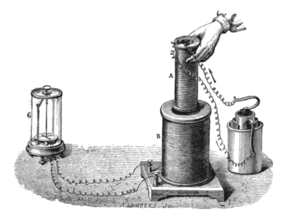
\includegraphics{Figures/faradayexp}
	\decoRule
	\caption[Faraday's Experiment]{Faraday's Experiment,\textsuperscript{\cite{poyser1918magnetism}}} which resulted in the law that was later used by Maxwell in making his equation.
	\label{fig:faradayexp}
\end{figure}

Equation \ref{eqn:amperesLaw} is also known as Ampère–Maxwell law, because although it originated from Ampère, the current form was derived by Maxwell to include the magnetic current density $\vec{J}$. The equation explains the effects of the magnetic field on the electric current.

Equation \ref{eqn:magneticDivergence}, otherwise known as Gauss's law for magnetism, talks about the divergence of the magnetic field. According to this law the divergence is always 0. What this means is that in a magnetic field there is no such thing as a source (positive divergence) or a sink (negative divergence), rather a magnetic field can be more closely compared to a closed loop that flows in one direction. That is why every magnet that we know of has two poles. To translate this into something more easily understandable, it basically means that, if we were to pick any subset of the area of a magnetic field, no matter what area we pick, we would have vector fields going inside this area, and vector fields going outside in equal number. A simple representation of this rule can be seen in \ref{fig:magneticdivergence}, where it can be noted that the number of vectors heading towards the north pole are equal to the vectors going outside of it. Interestingly enough, if the bar magnet were to be cut in half, then the result would be two smaller bar magnets with 2 poles each and the exact same vector field.

\begin{figure}
	\centering
	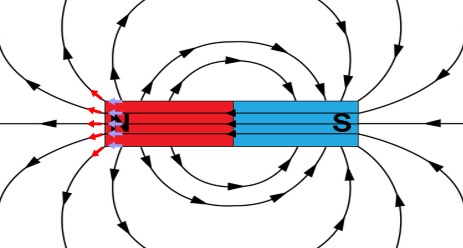
\includegraphics[scale=0.9]{Figures/magneticdivergence}
	\decoRule
	\caption[Magnetic Divergence]{A crude representation of magnetic divergence through the use of a bar magnet.}
	\label{fig:magneticdivergence}
\end{figure}

Equation \ref{eqn:gausslaw}, is the main Gauss law for electric currents. It looks rather similar to his law of magnetism on the left hand side; the previous magnetic divergence is now replaced with the electric divergence. The bigger difference is the $\rho$ on the right hand side, which is the density of charge of the electric field. In basic terms, it means that the divergence of the electric field is equal to the charge density for that point.

For the above equations, we also have the following material relations which will be useful later on:
\begin{equation}
	 \vec{D}(\vec{r},t) = \epsilon(\vec{r}) \cdot \vec{E}(\vec{r},t)
\end{equation}
\begin{equation}
	\vec{B}(\vec{r},t) = \mu(\vec{r}) \cdot \vec{H}(\vec{r},t)
\end{equation}

The equations above are shown in their derivative form, but they can also be shown as their integral equivalent. There is no difference in implementation, regardless of which form is used.

%-----------------------------------
%	SUBSECTION 2
%-----------------------------------

\subsection{Solving the Wave Equation}
Using the formulas above, we can derive the electromagnetic wave equation, which is needed to proceed with the implementation further. Firstly for convenience, we will assume that the environment is the vacuum of space. Secondly, we will also assume that there is no charge in this space. This means that $\epsilon(\vec{r})=\epsilon_{0}$ and $\mu(\vec{r})=\mu_{0}$. This allows us to simplify the above equations and give us the numerical solution for the wave equation

\begin{equation}
	\label{eqn:waveEquation}
	\Delta\vec{E}(\vec{r},t) - \frac{1}{c^2} \frac{\partial^2 \vec{E}(\vec{r},t)}{\partial t^2} = \mu_{0} \frac{\partial \vec{J}(\vec{r},t)}{\partial t},
\end{equation}

where: $$c = \frac{1}{\sqrt{\mu_{0}\epsilon_{0}}}$$

This equation is useful because it will be used to derive the formulas that are going to be needed for the simulations. Going forwards, this will be used as a basis to adapt our solution to every environment, regardless of dimensionality. From this point, there are many ways to proceed. Some of the most notable are the Finite Element Method (FEM), the Finite Integration Technique (FIT), and the Finite Difference Time Domain Method (FDTD). All of them are also known as Approximation Methods.

FEM is a well known numerical method used to obtain an approximation for a given boundary value problem. The basic principle is to divide a system into smaller subsets, called finite elements (hence the name), which are much simpler to solve. This is done by discretizing the given space for each of its dimensions, and then constructing a mesh of the object. As a result, from the initial boundary value problem we get a system of equations that are further used to approximate each singular simplified function over the given domain. These equations are then compiled together into a system of equations that is then used to model the initial problem. The solution is then approximated by solving this system and minimizing the error function.\textsuperscript{\cite{logan2011first}}

The finite integration technique (FIT) is a bit more straightforward. It can help numerically solve electromagnetic field problems by disctretizing in both the time and frequency domain. The first to introduce this technique was Thomas Weiland in 1977.\textsuperscript{\cite{weiland1977discretization}} It has later seen continuous improvements and can now cover all electromagnetic problems and applications. This approach works by using the Maxwell equations above and applying their integral form to a set of staggered grids (e.g. Cartesian grid). This allows for a memory efficient implementation as well as giving the ability to handle different boundary conditions and variable material properties.

Finally we have a well known computational electromagnetic technique used for approximation, the Finite Difference Time Domain Method. It is arguably the easiest method out of the three to understand and implement, which is surprising when considering the capabilities it has in solving wave equations. 

This simplicity is also the reason it was chosen for this thesis, as it is the only technique that one person can realistically implement by themselves in a reasonable time frame.\textsuperscript{\cite{davidson2010computational}} As the name implies this is a time-domain method, meaning that a wide range of frequencies can be covered with a single simulation run. The only caveat is that the time step needs to be small enough to not cause any instabilities in the system.

%----------------------------------------------------------------------------------------
%	SECTION 2
%----------------------------------------------------------------------------------------

\section{Finite Difference Time Domain Method}

FDTD was first proposed by Kane Yee in a 1966 paper and was initially called the Yee Algorithm, taken from the author's name. It was modified later from further research, resulting in the modern version that is widely used to this day. This method can be basically summarized in the following steps:

\begin{enumerate}
	\item Replace the derivatives from the Maxwell Equations with finite differences
	\item Discretize the space and time of the domain, while staggering the electric fields from the magnetic ones (e.g. by half a time step, and spatially by using a different axis)
	\item Get the update equations
	\item Use the update equations to get the future step for magnetic and electric fields
	\item Repeat the step above throughout the set duration
\end{enumerate}

The most important steps are 2 and 3, as the rest are relatively easy to do and it is highly unlikely for any mistakes to occur, especially once this is implemented in code. In the next section we will go quickly through the first step, which will the basis that will be used moving forward. Steps 2-5 are implementation specific and vary depending on the domain. As such, they will be explained for each scenario in their respective chapters.

\section{FDTD Implementation}

Before beginning with the discretization, we mentioned previously that Maxwell's Equations can be shown in both their differential form and their integral form:


\begin{equation}
	\label{eqn:electricinductionintegral}
	\oint E \cdot ds = - \frac{d}{dt} \int B \cdot dA
\end{equation}
\begin{equation}
	\label{eqn:amperesLawintegral}
	\oint H \cdot ds = \int \frac{dD}{dt} \cdot dA
\end{equation}
\begin{equation}
	\label{eqn:magneticDivergenceintegral}
	\int D \cdot dA = \int \rho dV
\end{equation}
\begin{equation}
	\label{eqn:gausslawintegral}
	\int B \cdot dA = 0
\end{equation}

The material relations would look as follows:

\begin{equation}
	\label{eqn:dIntegral}
	D = \epsilon \cdot E
\end{equation}
\begin{equation}
	\label{eqn:bIntegral}
	B = \mu \cdot H
\end{equation}

By plugging \ref{eqn:bIntegral} and \ref{eqn:dIntegral} into equations \ref{eqn:electricinductionintegral} and \ref{eqn:amperesLawintegral} respectively, we get:

\begin{equation}
	\label{eqn:electricUpdateIntegral}
	\oint E \cdot ds = - \frac{d}{dt} \int \mu \cdot H \cdot dA
\end{equation}
\begin{equation}
	\label{eqn:magneticUpdateIntegral}
	\oint H \cdot ds = \frac{d}{dt} \iint \epsilon \cdot E \cdot dA
\end{equation}

Equations \ref{eqn:electricUpdateIntegral} and \ref{eqn:magneticUpdateIntegral} are going to be used later on during the implementation to derive the specific update equations. With all that, the general theoretical part is finished. For this project, we will need to implement the above functions into a program that can generate approximate data on electromagnetic waves, which will be discussed in the next section.

\subsection{Application Requirements}

The result of this project is not only this documentation, but also a relatively simple program that can be used either as is, or implemented into a bigger project with minor adjustments. As such, the resulting application must adhere to the following requirements:

\begin{itemize}
	\item Allow for the generation of electromagnetic data in a set environment (e.g. vacuum)
	\item Have a smooth impulse to start off the simulation
	\item Use only the default C++ libraries, no external dependencies
	\item Support one dimensional, two dimensional, and three dimensional domains.
	\item Be simple and compact, so that it can be adapted to a bigger application if necessary
\end{itemize}

The first requirement is understandably the most basic functionality, the goal of the whole project. This data will be generated from scratch, using the environment variables of permittivity $\epsilon$ and permeability $\mu$. These values can be changed depending on the environment, which can be vacuum, copper, etc. The examples here will use the values for free space $\epsilon_{0}$ and $\mu_{0}$. Also, these values are going to be constant throughout the simulation, meaning we will have one material through out the whole domain. 

Without a starting impulse, there would be nothing to simulate, as the data would simply keep its initial value of zero. If we were to add an immediate pulse of an arbitrary value to a single point, it would prove sufficient. However, this would result in a sudden explosion of a single electromagnetic pulse that would simply travel along the domain as a single point, thus providing us with a near useless visualization once the data is put into an appropriate program. 

Instead, we can use a Gaussian pulse excitation in the middle of the domain, and have it propagate throughout it. This is ideal because we are using reflective boundaries, meaning the pulse will bounce back and forth between each boundary without any loss. If we were to use absorbing boundary conditions, such an excitation would eventually lead to the waves disappearing completely. For such cases, a steady sinusoidal excitation that keeps going would prove more interesting.

We will be using a Gaussian pulse for our example. The generic formula is given below:

\begin{equation}
	\label{eqn:gaussianPulse}
	f(t) = \alpha e^{-\beta(t - T_\varepsilon/2)^2}
\end{equation}
where
\begin{equation}
	\label{eqn:gaussianBeta}
	\beta = - (\frac{2}{T_\varepsilon})^2 \ln\varepsilon
\end{equation}

A good value for sufficient smoothness would be $\varepsilon = 0.001$, but this is heavily dependent on the implementation.

For the third requirement, the reason why we would want to avoid the use of libraries that are not included by default in C++ is that such libraries could make the program dependent on the operating system that the machine is running, PATH variables, etc. In short, it would complicate the setup to run such a program too much, possibly voiding the last requirement. On top of that, in insisting on using only the very basics that C++ has to offer, the resulting code will be easier to relate to the formulas that are shown in this thesis, since all the code will be visible at all times. With that said, various improvements could be made if the use of external libraries is allowed. That will be discussed in more details in the Conclusion.

Fourth, we want the application to support anything from one to three dimensions. While only a 3D simulation would be realistically desired, for a thesis the 1D and 2D scenarios are also interesting to study. Not only that, but the 1D application leads smoothly to the development of the 2D application, which in turn leads to the smooth development of the 3D application. This progression resulted in having a standalone program for each scenario, rather than one for all of them. Rather than unify these applications, they were intentionally left as separate programs in the end, because it helps in complying with the last requirement.

Lastly, after going through each of the previous requirements, this one is rather self-explanatory. To begin with, simple and compact code that works well standalone is one of the most important programming practices that developers should follow. While this program's goal is to simply be used as a demonstration of such an implementation, it should also be easily modifiable and adaptable, so that it can provide a good basis that can be used by larger applications that include far more features.

With that said, we will have to go through certain limitations that plague all computers simply due to their nature. Since these limitations cannot be bypassed as of yet, we can never achieve an exact, perfectly realistic simulation. Thus, it is good to keep them in mind while developing such applications.

\subsection{Computational Limitations and Inaccuracies Explained}

Programmers can use programming languages to instruct computers to perform certain commands in certain orders, thus creating applications. However, these instructions are not what the computers use to dictate what should happen. These programming languages are decoded by the interpreter of choice, and then passed down in the form of a lower level language. This process can occur more than once too, until we get to the smallest unit a computer can have: a bit.

A bit is simple; it can have either a value of zero or one. Instructions are basically translated into many such bits, thus making what is basically computer language. Each instruction could be translated into millions of bits, but that by itself would not cause issues normally. The issue is that, no matter how powerful the computer is or how much memory it has, these bits are finite. As such, they present limitations when dealing with infinite concepts.

One such concept is infinite numbers. To best explain this, let us use an example: summing thirds into a whole. If a person was to be asked to add $\frac{1}{9}$ nine times, they would do the following:
$$\frac{1}{9} + \frac{1}{9} + \frac{1}{9} + \frac{1}{9} + \frac{1}{9} + \frac{1}{9} + \frac{1}{9} + \frac{1}{9} + \frac{1}{9} = 1 \;,$$ which we know is correct. However, when we run the following code snippet:

\begin{minted}[breaklines,frame=single]{c++}
	double a = 1.0/9.0;
	if (a + a + a + a + a + a + a + a + a == 1.0) {
		cout << "Equal to 1";
	} else {
		cout << "Not equal";
	}
\end{minted}

we would get the following result (Fig. \ref{fig:finiteprecision}): 
\begin{figure}[h!]
	\centering
	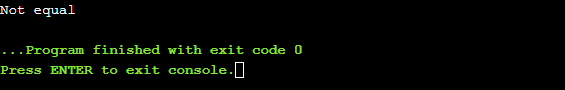
\includegraphics{Figures/finiteprecision}
	\decoRule
	\caption[Code Result]{According to our code, the total sum is not equal to 1.0, even though it should be.}
	\label{fig:finiteprecision}
\end{figure}

What is happening is that we are asking a computer to store the infinite number $1/9 = 0.\overline{1}$ using a finite amounts of bit. Depending on the data type we use, we can have anywhere from 8 bits of precision, to $2^8$ bits. However, that is still a finite amount, and no matter what we do the resulting value will be truncated to $0.1111...1$, resulting in a sum of $0.9999...9 \neq 1.0$ . That is why any simulation, regardless of the computer or the method used, will always be an approximation of reality. When performing thousands of calculations, this margin of error increases further. Despite that, these approximations are enough to give us a good idea of what to expect.
% Chapter Template

\chapter{FDTD - One-Dimensional Scenario} % Main chapter title

\label{Chapter2} % Change X to a consecutive number; for referencing this chapter elsewhere, use \ref{ChapterX}

In this chapter, we will go more in depth into developing an application that can generate electromagnetic data in a one-dimensional domain. In the previous chapter, we mentioned a series of steps to implement FDTD, and that a part of them depend on the particular implementation. A keen eye will notice moving forward, that while the code will not change too much, each implementation deserves a different approach.

%----------------------------------------------------------------------------------------
%	SECTION 1
%----------------------------------------------------------------------------------------

\section{1D Discretization}



%-----------------------------------
%	SUBSECTION 1
%-----------------------------------
\subsection{Subsection 1}



%-----------------------------------
%	SUBSECTION 2
%-----------------------------------

\subsection{Subsection 2}


%----------------------------------------------------------------------------------------
%	SECTION 2
%----------------------------------------------------------------------------------------

\section{C++ Implementation}

\begin{minted}[breaklines,frame=single]{c++}
#define _USE_MATH_DEFINES

#include <iostream>
#include <stdio.h>
#include <math.h>
#include <stdlib.h>
#include <cmath>
#include <vector>
#include <string>

using namespace std;

const double permitivity = 8.854e-12;
const double permeability = 1.256e-6;

double L = 5;
int N = 200;
int iterNum = 800;
//double deltaX = L / N;
//double deltaY = L / N;
double deltaZ = L / N;
double deltaT = (deltaZ * sqrt(permitivity*permeability));

// variables needed for Gaussian Pulse excitation
double eps = 1e-3;
double Teps = 50 * deltaT;
double beta = -(pow((2/Teps), 2) * log(eps));


vector<double> E;
vector<double> H;
vector<double> tE;
vector<double> tH;

int main()
{
	E.assign(N, 0);
	H.assign(N, 0);
	
	
	for(int i = 0; i < iterNum; i++) {
		
		double t = i * deltaT;
		double gamma = Teps / 2;
		
		E[0] = exp(-(beta * pow((t - gamma), 2)));  //TO-DO: Gaussian excitation, alpha = 1, Teps = 50*deltaT, eps = 1e-3, t = i * deltaT
		
		// loop for values
		for (int z = 0; z < N-1; z++) {
			H[z] = H[z] - (deltaT / permeability / deltaZ) * (E[z] - E[z+1]);
		}
		
		for (int z = 1; z < N-1; z++) {
			E[z] = E[z] + (deltaT / permitivity / deltaZ) * (H[z] - H[z-1]);
		}
		
		
		// time graph
		tE.push_back(E[100]);
		tH.push_back(H[100]);
	}
	
	
	cout << "\n\ntE\n";
	
	// print E values
	for (int n = 0; n < iterNum; n++) {
		cout << to_string(tE[n]) + ",";
	}
	
	cout << "\n\ntH\n";
	
	// print H values
	for (int n = 0; n < iterNum; n++) {
		cout << to_string(tH[n]) + ",";
	}
	
}
\end{minted}

\section{Data Visualization}

\begin{figure}
	\centering
	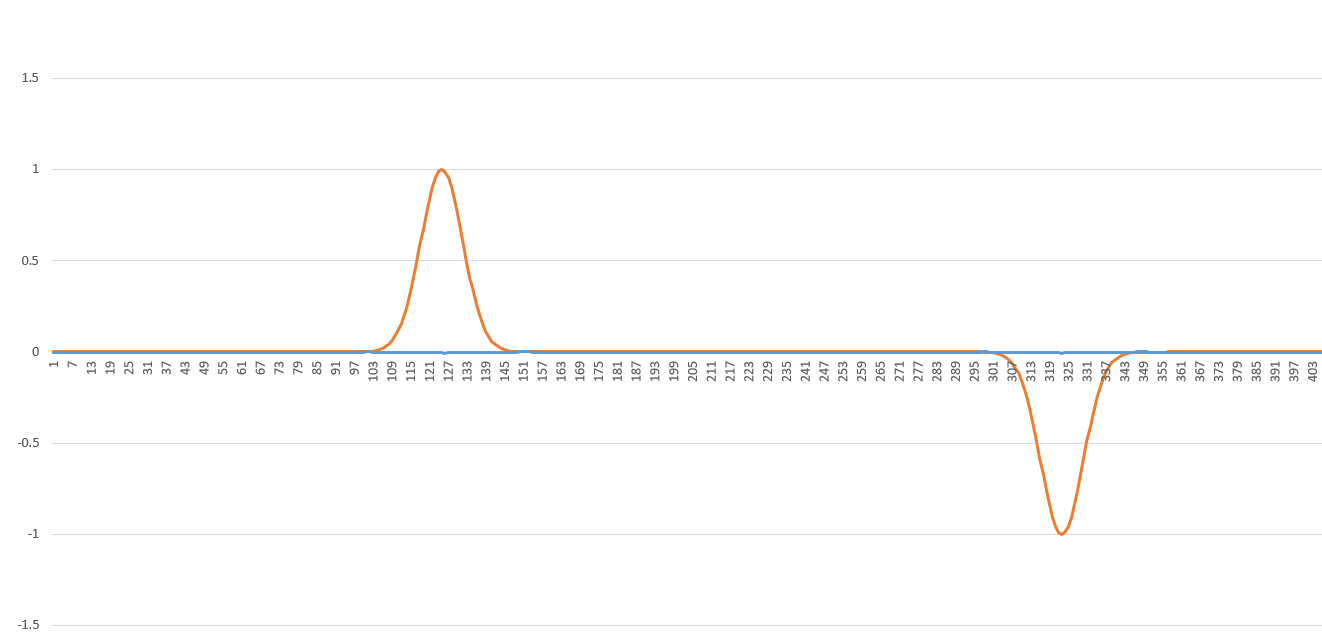
\includegraphics[scale=0.75]{Figures/1DtimeGraph1}
	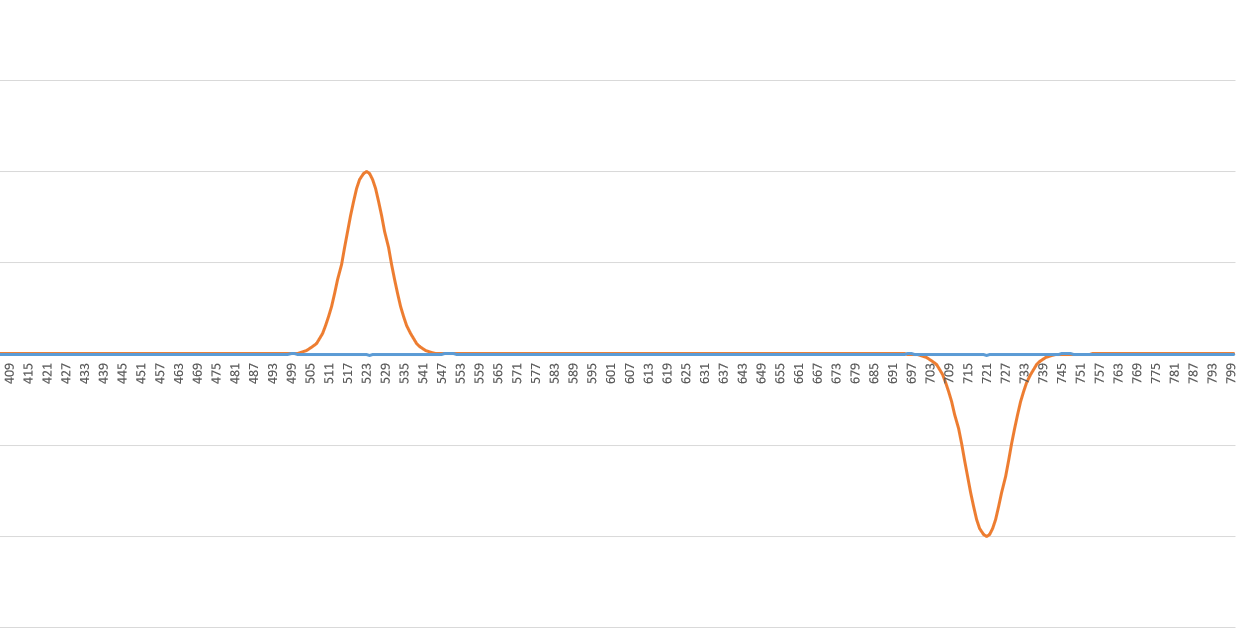
\includegraphics[scale=0.8]{Figures/1DtimeGraph2}
	\decoRule
	\caption[1D Electromagnetic Time Graph]{The time graph of the electromagnetic data generated by our 1D application.}
	\label{fig:emTimeGraph}
\end{figure}

\begin{figure}
	\centering
	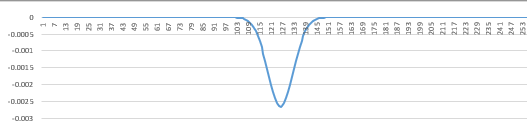
\includegraphics{Figures/1DmagneticTimeSnippet}
	\decoRule
	\caption[1D Magnetic Time Snippet]{A snippet of the time graph shown in Figure \ref{fig:emTimeGraph} zoomed in}
	\label{fig:mTimeSnippet}
\end{figure} 
% Chapter Template

\chapter{FDTD - Two-Dimensional Scenario} % Main chapter title

\label{Chapter3} % Change X to a consecutive number; for referencing this chapter elsewhere, use \ref{ChapterX}

%----------------------------------------------------------------------------------------
%	SECTION 1
%----------------------------------------------------------------------------------------

\section{Main Section 1}

%-----------------------------------
%	SUBSECTION 1
%-----------------------------------
\subsection{Subsection 1}
%-----------------------------------
%	SUBSECTION 2
%-----------------------------------

\subsection{Subsection 2}
%----------------------------------------------------------------------------------------
%	SECTION 2
%----------------------------------------------------------------------------------------

\section{C++ Implementation}

\begin{minted}[breaklines,frame=single]{c++}
	double L = 5;
	int N = 200;
	int iterNum = 800;
	double deltaX = L / N;
	double deltaY = L / N;
	double deltaZ = L / N;
	double deltaT = (deltaZ * sqrt(permitivity*permeability)  * (1/sqrt(2))); // 1/C * 1/sqrt2 * deltaZ
	
	// variables needed for Gaussian Pulse excitation
	double eps = 1e-3;
	double Teps = 50 * deltaT;
	double beta = -(pow((2/Teps), 2) * log(eps));
	
	
	vector<vector<double>> Ex(N, vector<double> (N, 0));
	vector<vector<double>> Ey(N, vector<double> (N, 0));
	vector<vector<double>> Hz(N, vector<double> (N, 0));
	
	const string filePath = "./Out/";
	
	void writeEDataToCsvFile(string filename, vector<vector<double>> Ex, vector<vector<double>> Ey){
		
		//	"x","y",Ex,Ey
		//	0,0,Ex[x,y],Ey[x,y]
		
		ofstream csvFile(filename);
		csvFile << "x,y,z,Ex,Ey\n";
		
		for (int x = 0; x < Ex[0].size(); x++) {
			for (int y = 0; y < Ex[x].size(); y++) {
				csvFile << to_string(x) + "," + to_string(y) + ",0," + to_string(Ex[x][y]) + "," + to_string(Ey[x][y]) + "\n";
			}
		}
		
		csvFile.close();
	}
	
	void writeHDataToCsvFile(string filename, vector<vector<double>> Hz){
		
		//	"x","y",Hz
		//	0,0,Hz[x,y]
		
		ofstream csvFile(filename);
		csvFile << "x,y,z,Hz\n";
		
		for (int x = 0; x < Hz[0].size(); x++) {
			for (int y = 0; y < Ex[x].size(); y++) {
				csvFile << to_string(x) + "," + to_string(y) + ",0," + to_string(Hz[x][y]) + "\n";
			}
		}
		
		csvFile.close();
	}
	
	int main()
	{
		for(int i = 0; i < iterNum; i++) {
			
			double t = i * deltaT;
			double gamma = Teps / 2;
			
			// reducing the magnitude since in free space
			Hz[99][99] = exp(-(beta * pow((t - gamma), 2))) * 10e-4;  //TO-DO: Gaussian excitation, alpha = 1, Teps = 50*deltaT, eps = 1e-3, t = i * deltaT
			
			for (int i = 0; i < N-1; i++) {
				for (int j = 1; j < N-2; j++) {
					Ex[i][j] = Ex[i][j] + (deltaT / permitivity / deltaZ) * (Hz[i][j] - Hz[i][j-1]);
				}
			}
			
			for (int i = 1; i < N-2; i++) {
				for (int j = 0; j < N-1; j++) {
					Ey[i][j] = Ey[i][j] - ((deltaT / permitivity / deltaZ) * (Hz[i][j] - Hz[i-1][j]));
				}
			}
			
			writeEDataToCsvFile((filePath + "E/E.csv." + to_string(i)), Ex, Ey);
			
			// loop for values
			for (int i = 0; i < N-1; i++) {
				for (int j = 0; j < N-1; j++) {
					Hz[i][j] = Hz[i][j] - ((deltaT / permeability / deltaZ) * (Ex[i][j] - Ex[i][j+1] + Ey[i+1][j] - Ey[i][j]));
				}
			}
			
			
			writeHDataToCsvFile((filePath + "H/H.csv." + to_string(i)), Hz);
			
		}
	}
\end{minted}


\section{Data Visualization}

\begin{figure}
	\centering
    \begin{subfigure}{.49\textwidth}
    	\centering
    	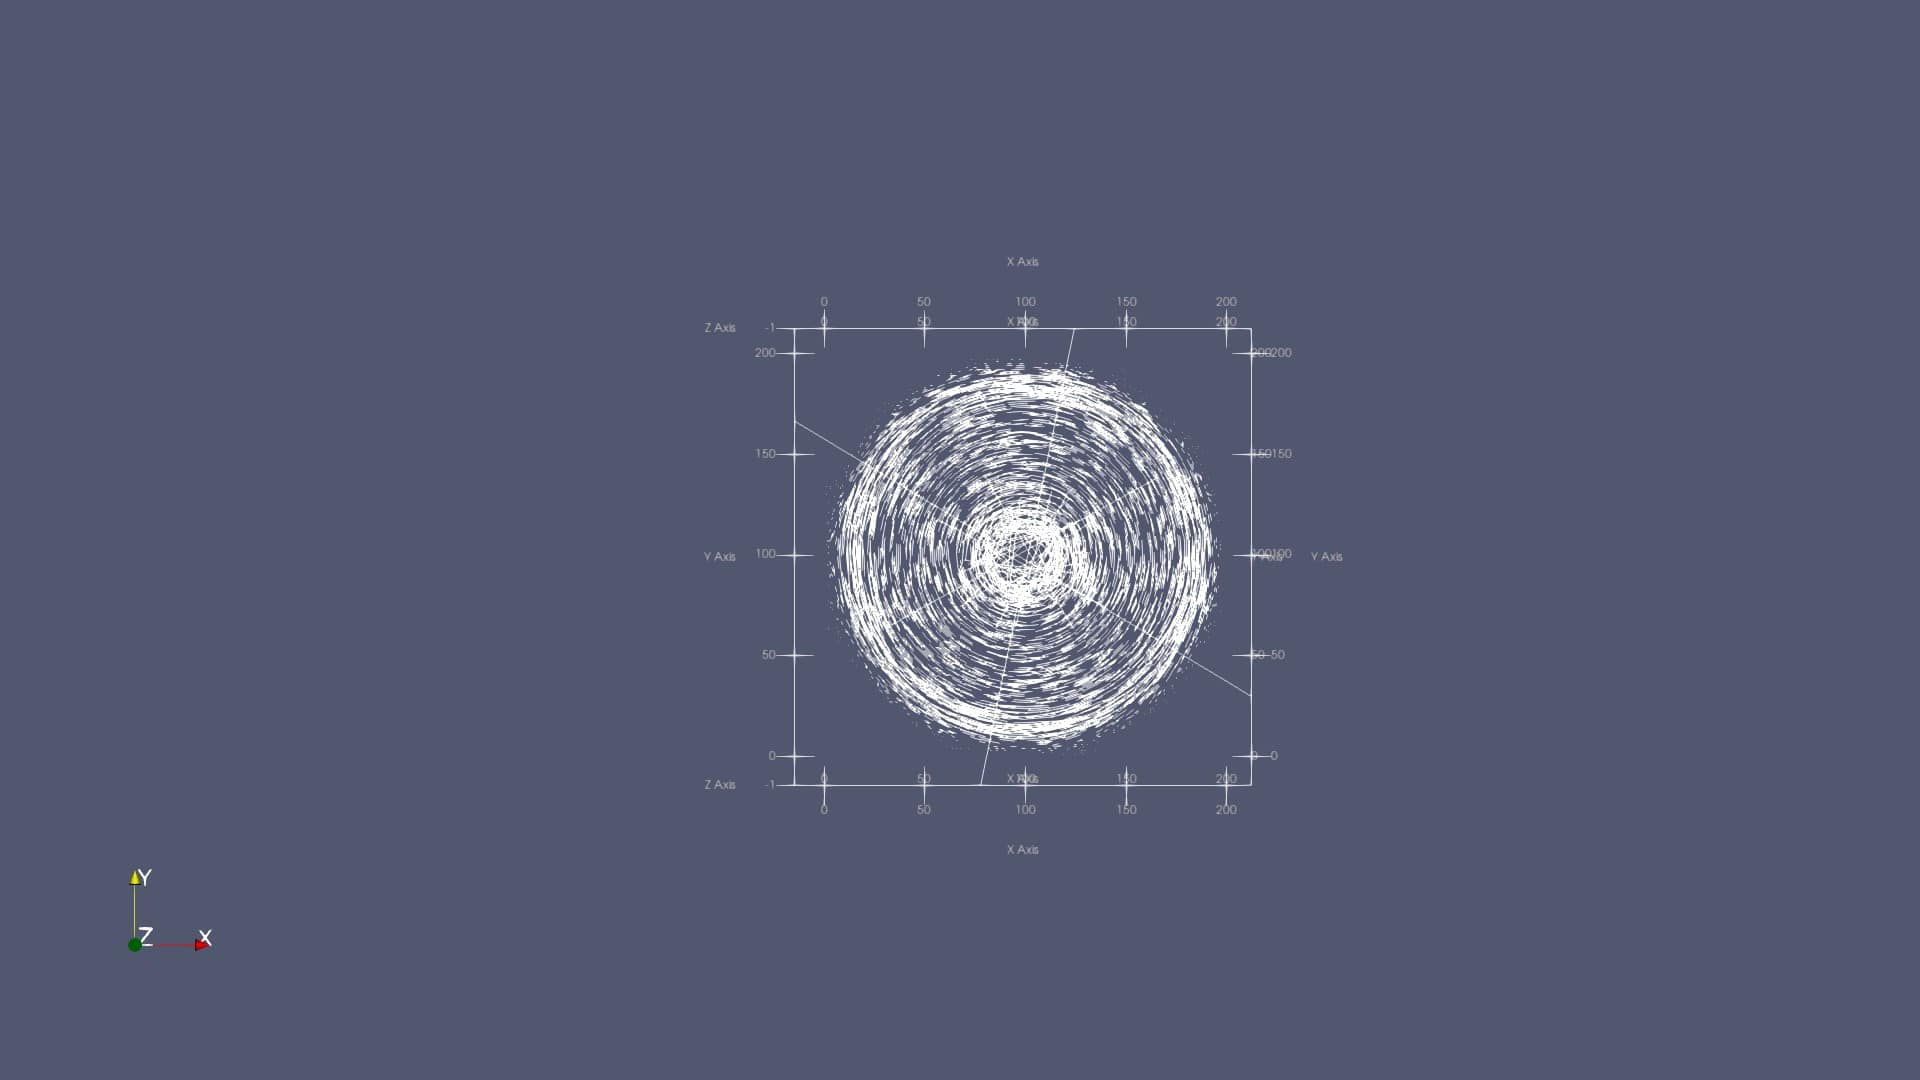
\includegraphics[width=.95\linewidth]{Figures/FDTD2DE1}
    	\caption{t = 200}
    \end{subfigure}
    \begin{subfigure}{.49\textwidth}
    	\centering
    	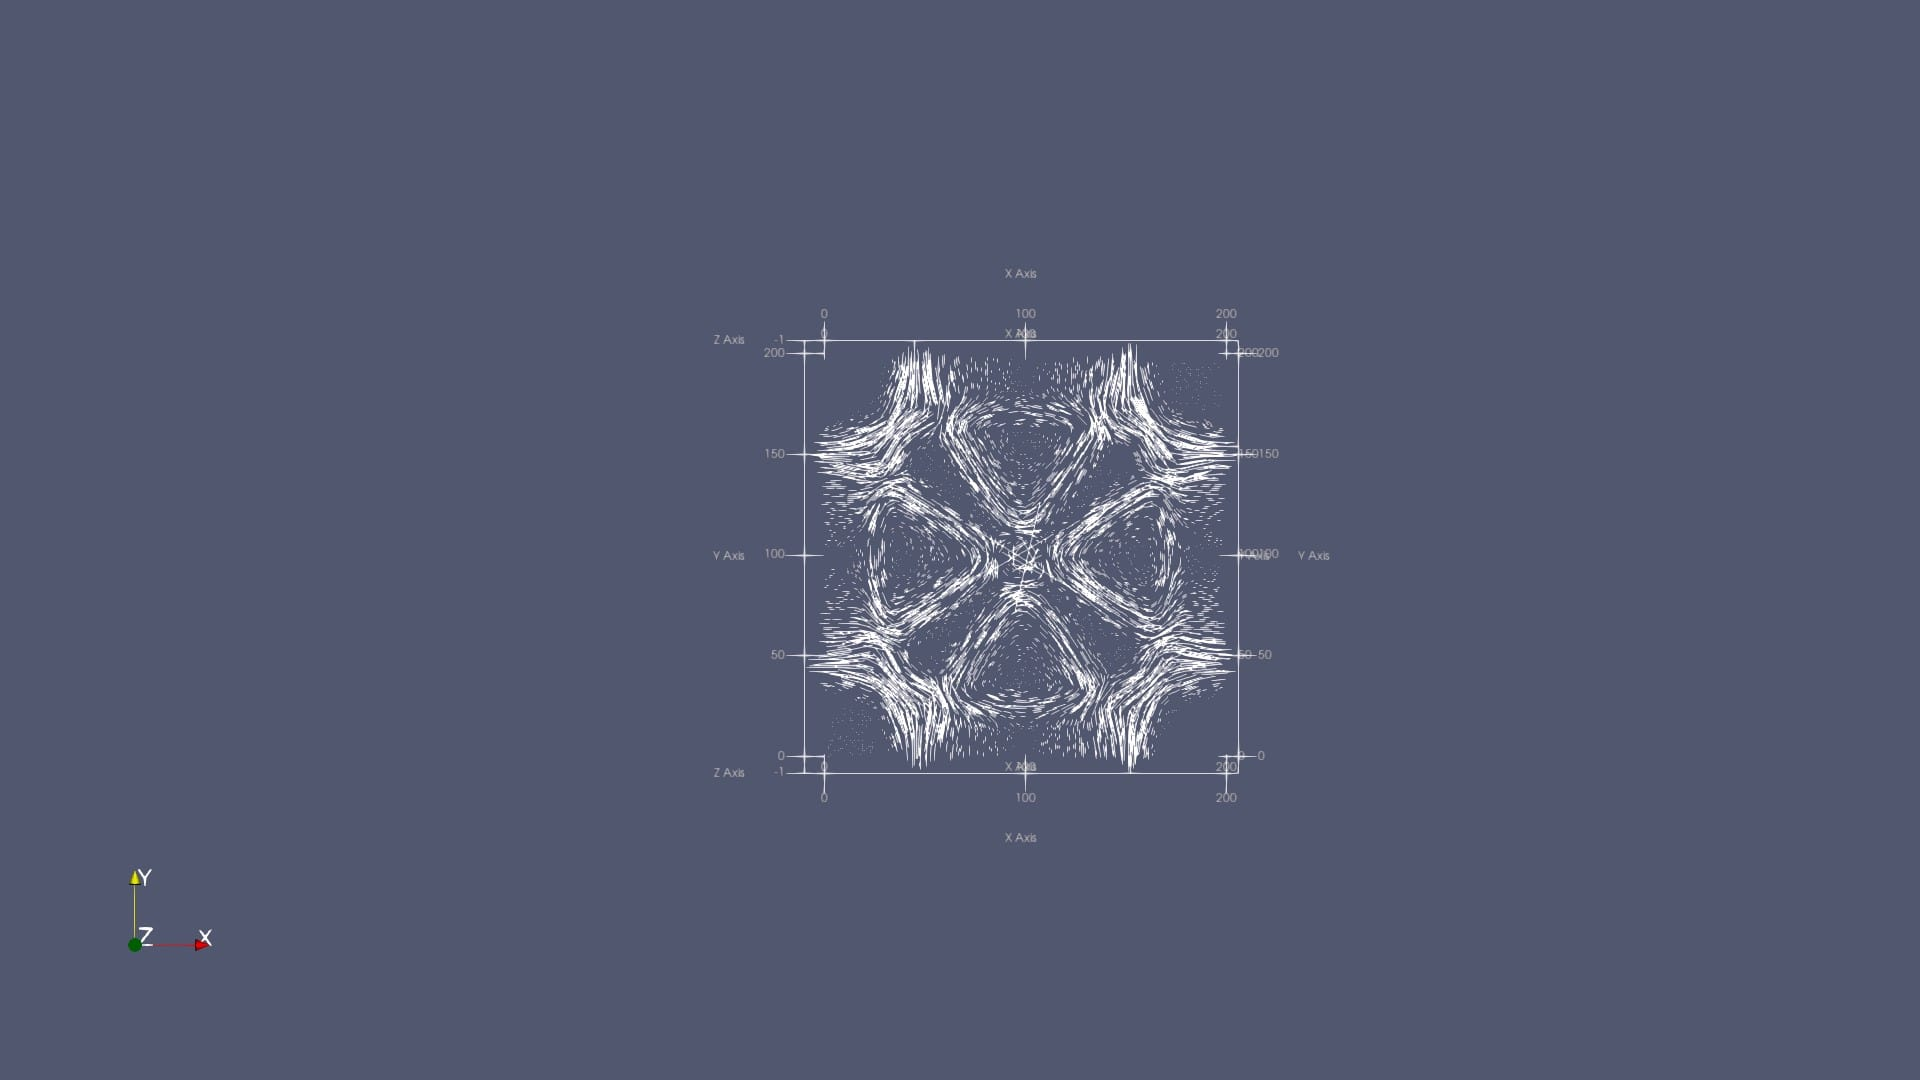
\includegraphics[width=.95\linewidth]{Figures/FDTD2DE2}
    	\caption{t = 400}
    \end{subfigure}
    \begin{subfigure}{.49\textwidth}
    	\centering
    	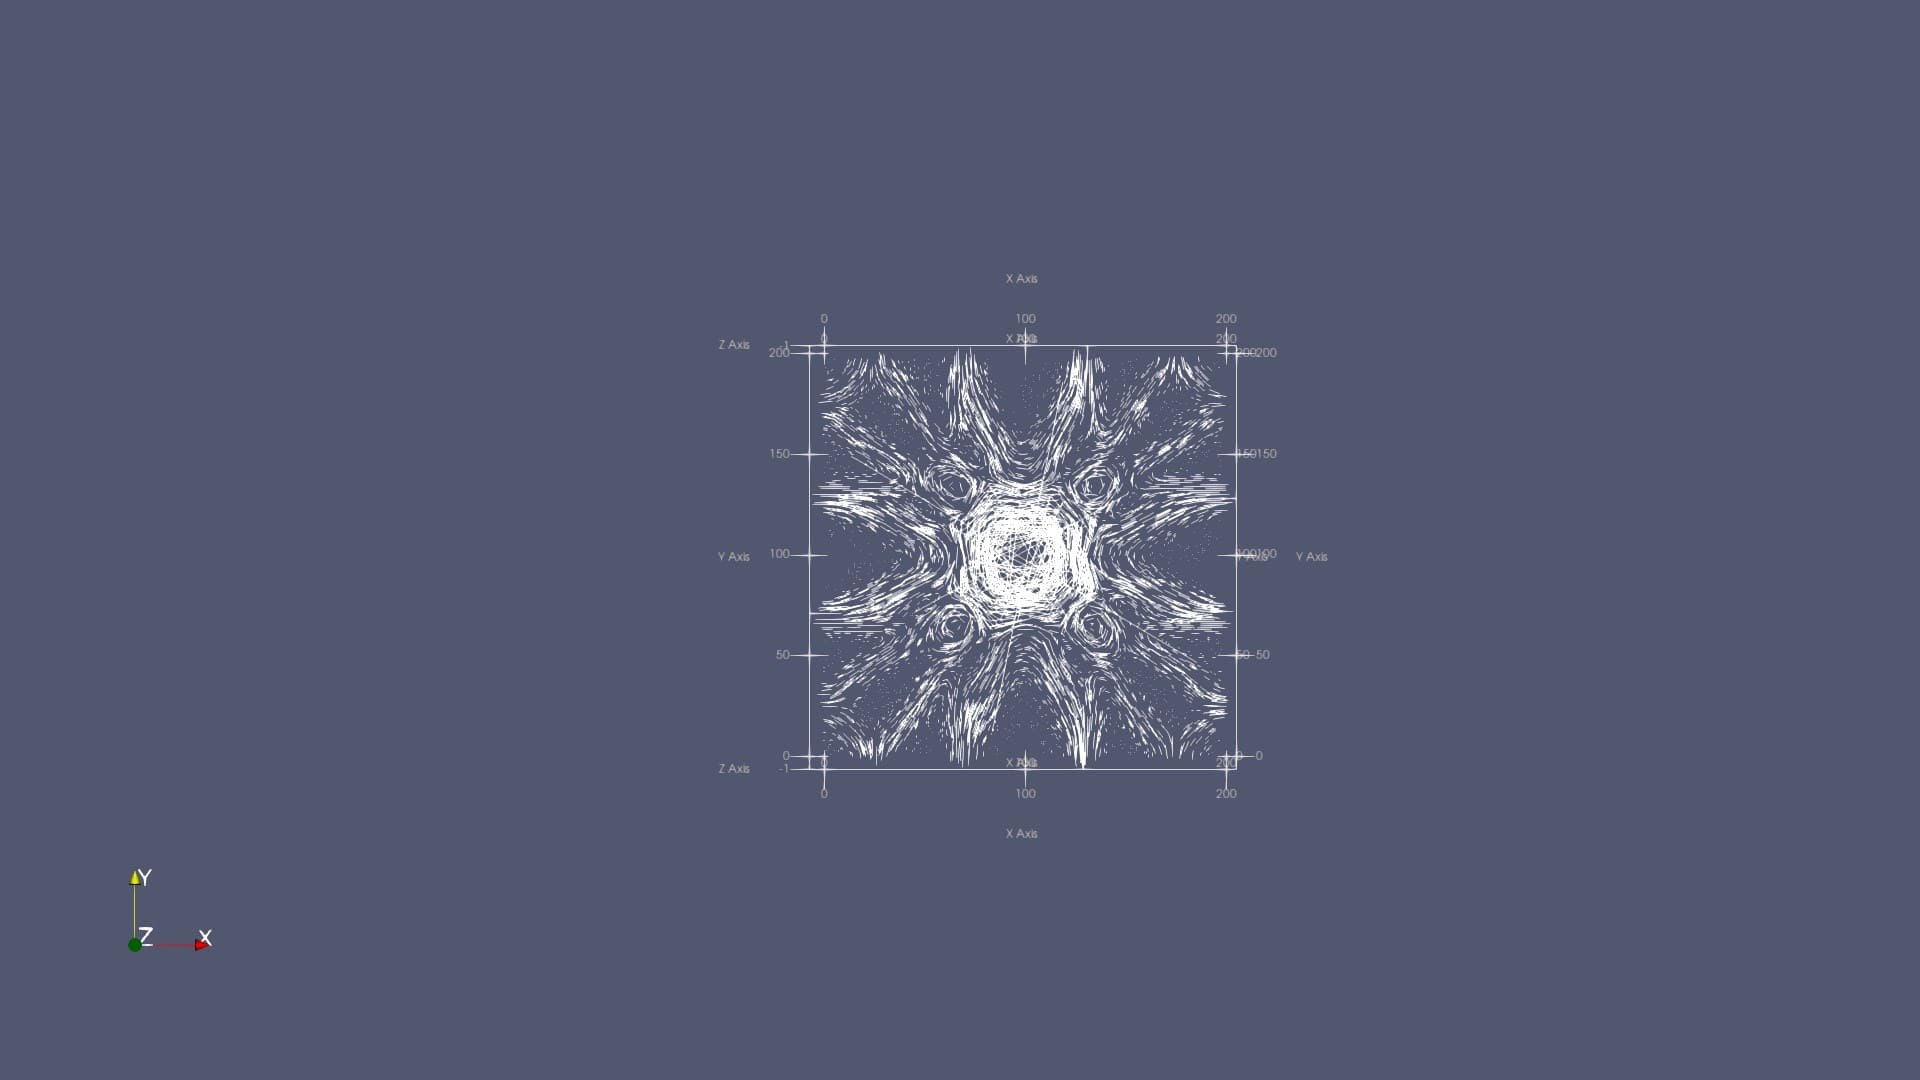
\includegraphics[width=.95\linewidth]{Figures/FDTD2DE3}
    	\caption{t = 600}
    \end{subfigure}
    \begin{subfigure}{.49\textwidth}
    	\centering
    	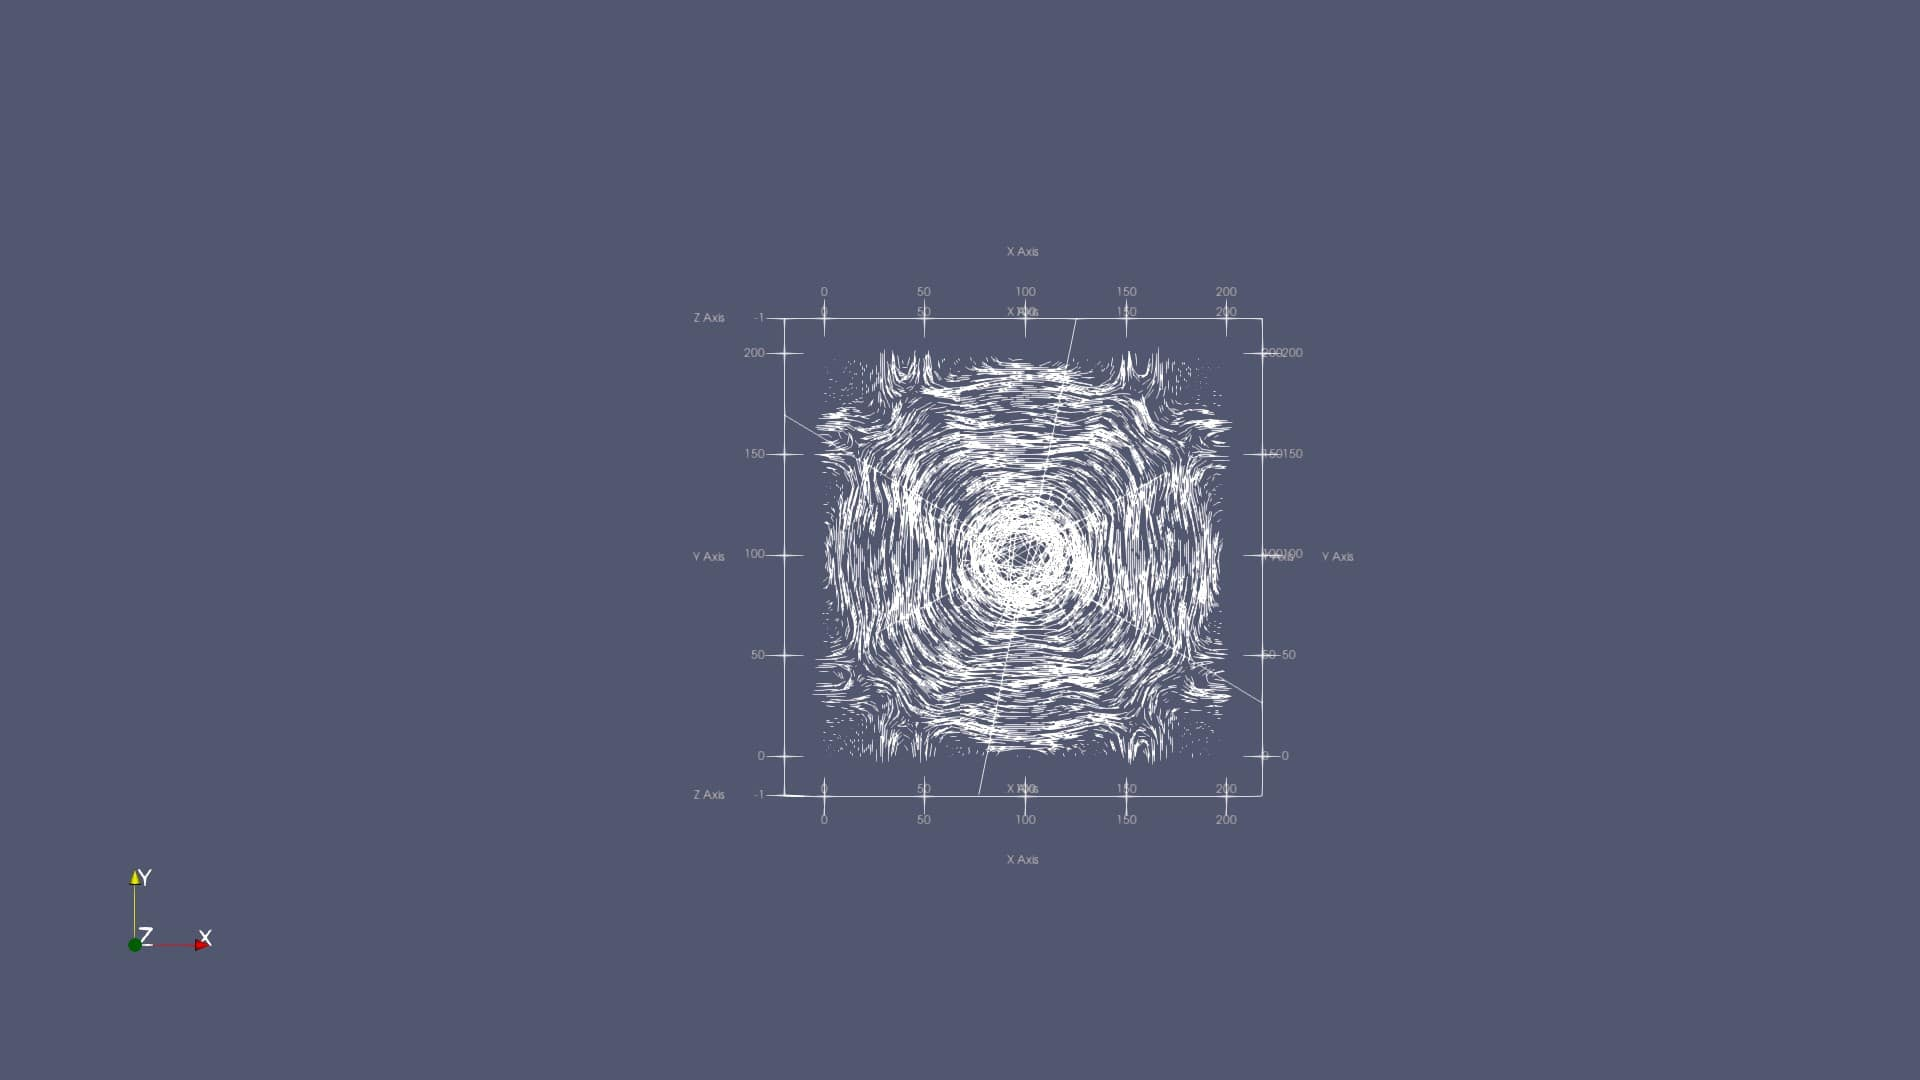
\includegraphics[width=.95\linewidth]{Figures/FDTD2DE4}
    	\caption{t = 800}
    \end{subfigure}
	\decoRule
	\caption[2D Electric Field Simulation]{A simulation of the 2D electric field.}
	\label{fig:FDTD2DE}
\end{figure}

\begin{figure}
	\centering
	\begin{subfigure}{.49\textwidth}
		\centering
		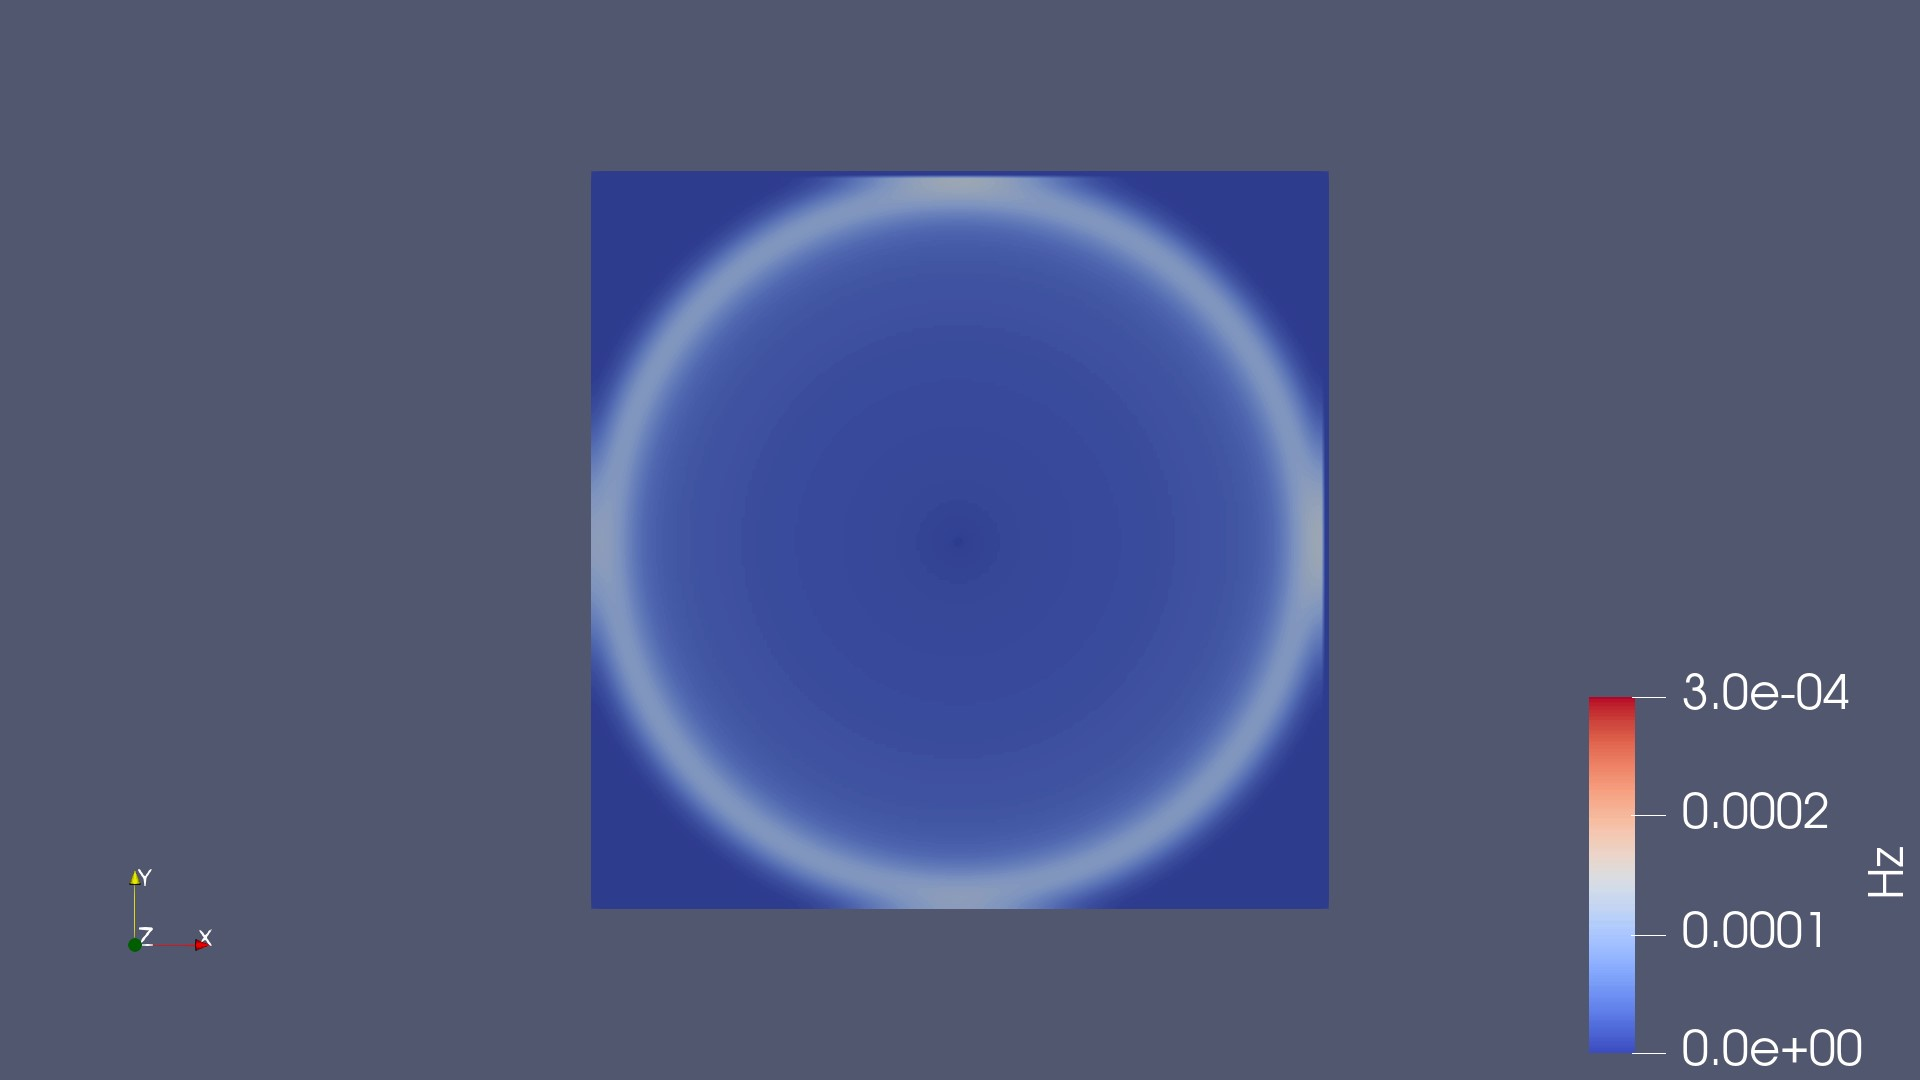
\includegraphics[width=.95\linewidth]{Figures/FDTD2DH1}
		\caption{t = 200}
	\end{subfigure}
	\begin{subfigure}{.49\textwidth}
		\centering
		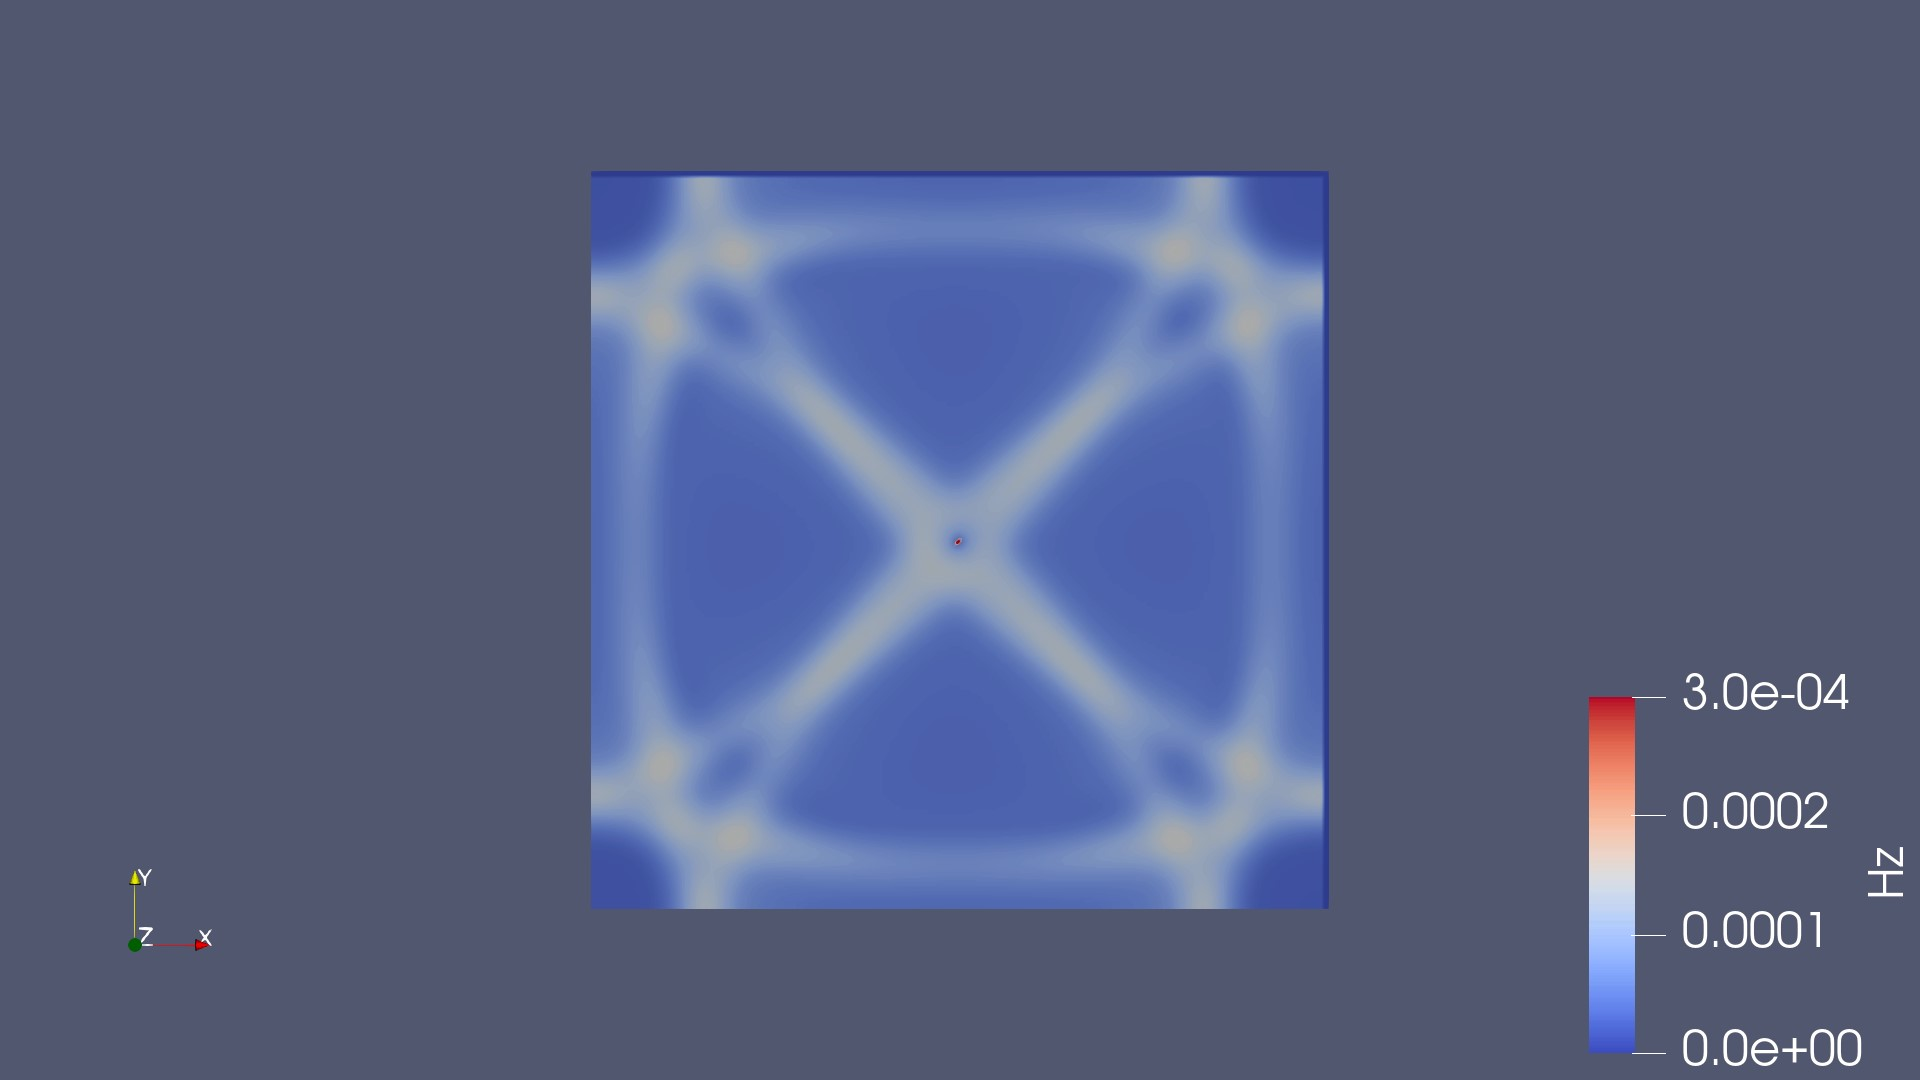
\includegraphics[width=.95\linewidth]{Figures/FDTD2DH2}
		\caption{t = 400}
	\end{subfigure}
	\begin{subfigure}{.49\textwidth}
		\centering
		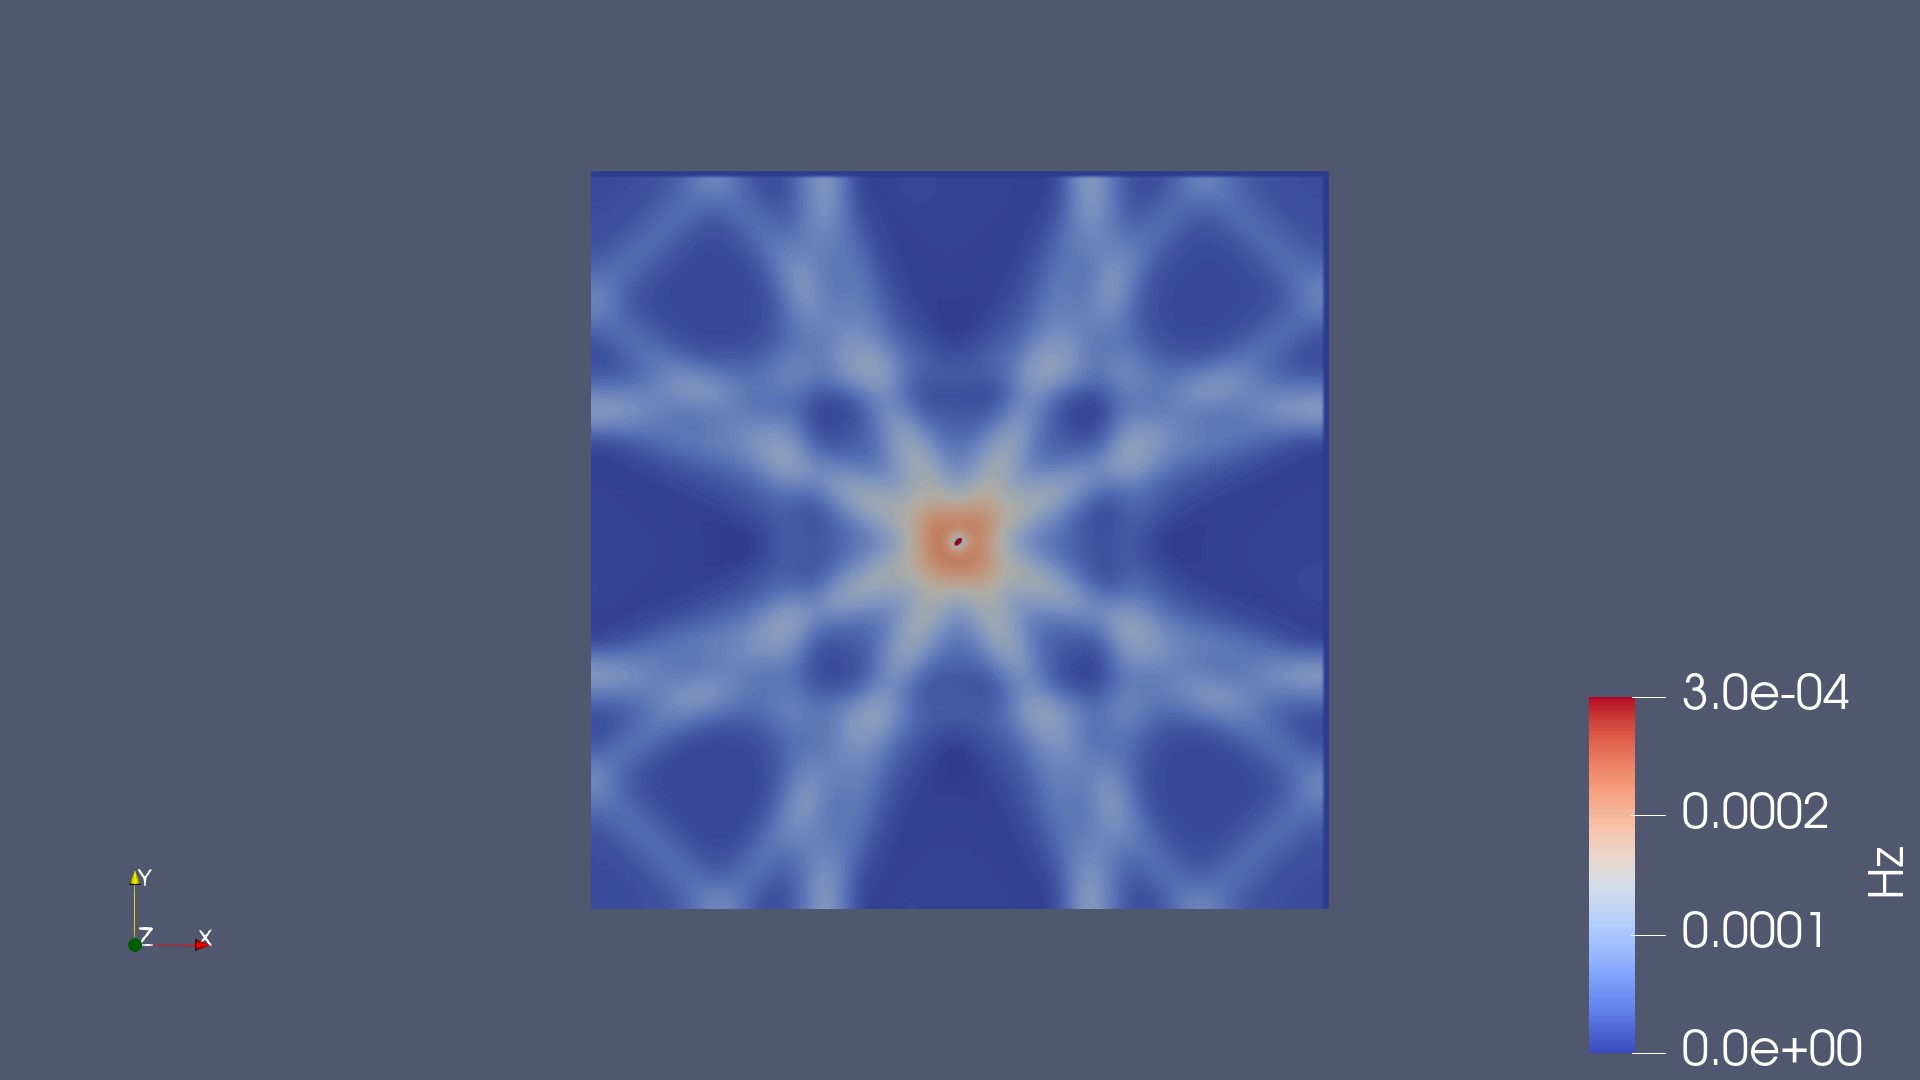
\includegraphics[width=.95\linewidth]{Figures/FDTD2DH3}
		\caption{t = 600}
	\end{subfigure}
	\begin{subfigure}{.49\textwidth}
		\centering
		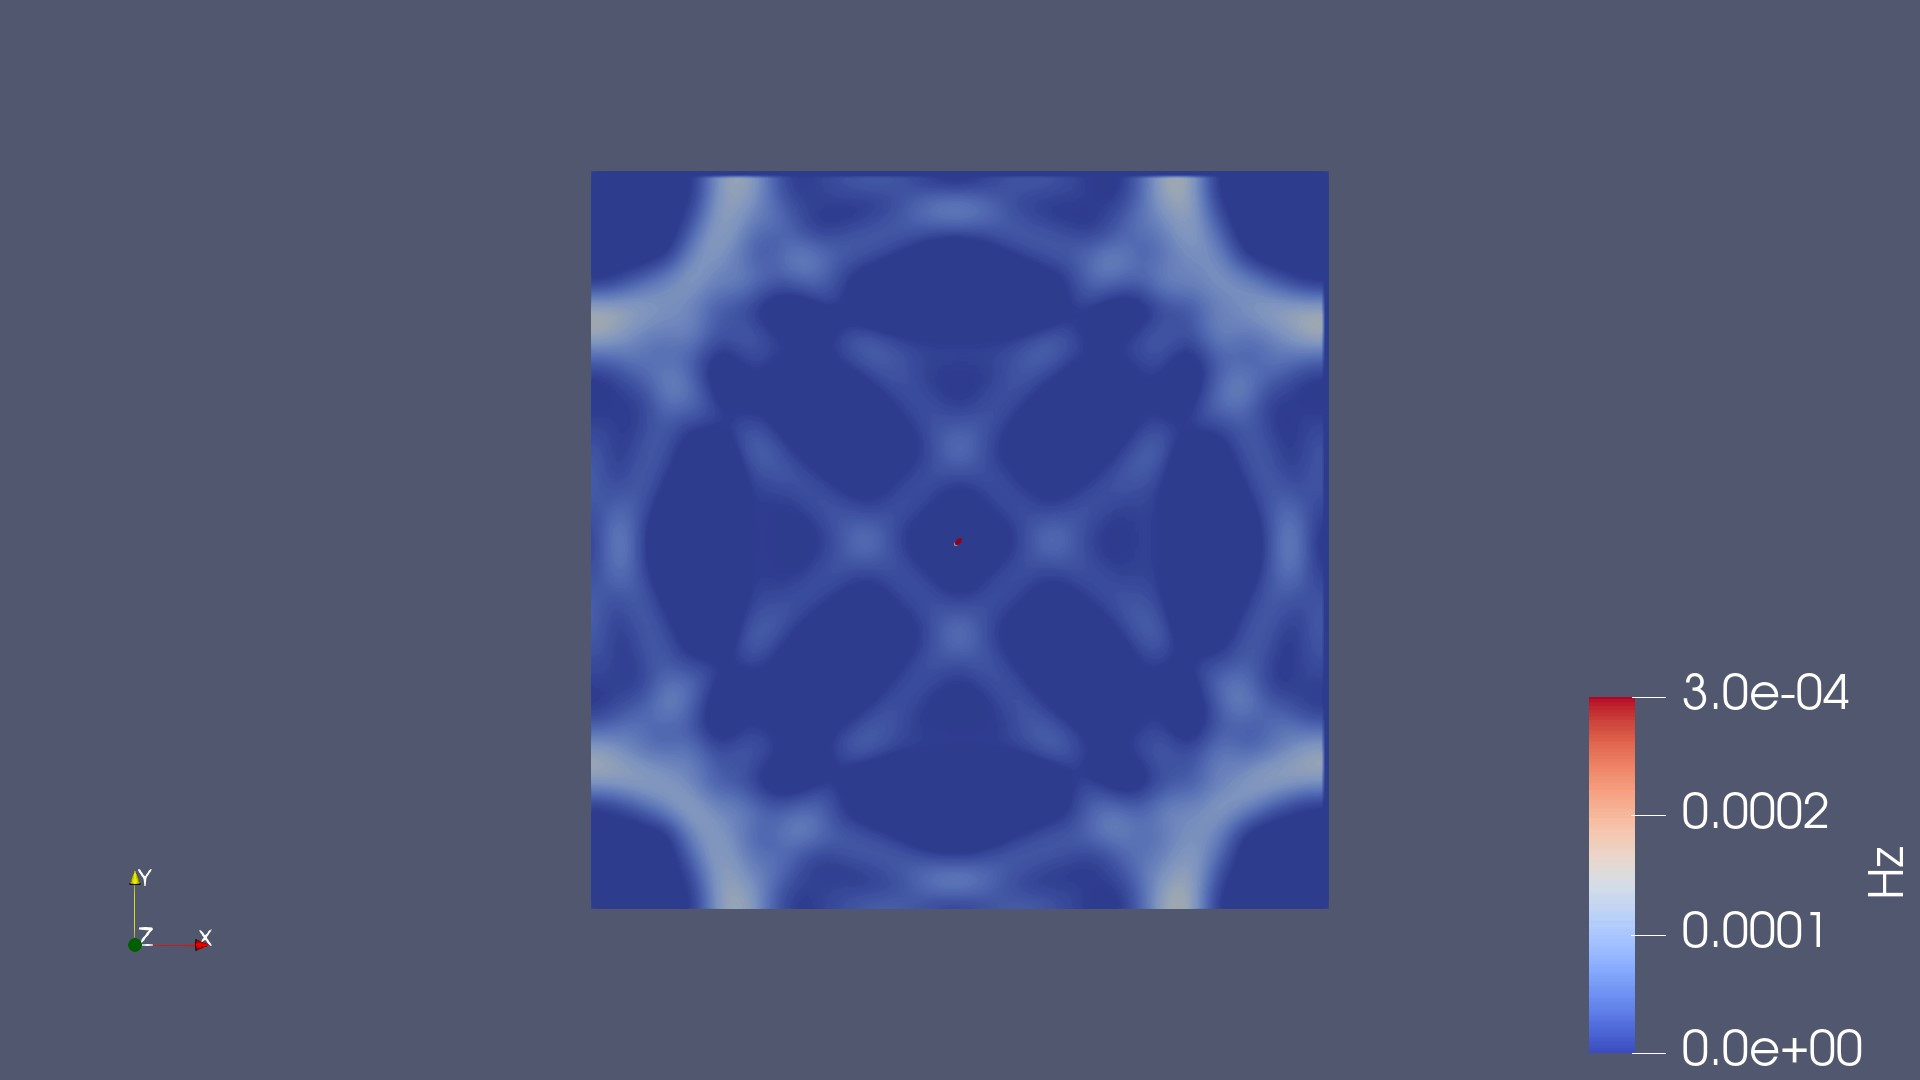
\includegraphics[width=.95\linewidth]{Figures/FDTD2DH4}
		\caption{t = 800}
	\end{subfigure}
	\decoRule
	\caption[2D Magnetic Field Simulation]{A simulation of the 2D magnetic field.}
	\label{fig:FDTD2DH}
\end{figure}
% Chapter Template

\chapter{FDTD - 3 Dimensional Scenario} % Main chapter title

\label{Chapter4} % Change X to a consecutive number; for referencing this chapter elsewhere, use \ref{ChapterX}

%----------------------------------------------------------------------------------------
%	SECTION 1
%----------------------------------------------------------------------------------------

\section{Main Section 1}

Lorem ipsum dolor sit amet, consectetur adipiscing elit. Aliquam ultricies lacinia euismod. Nam tempus risus in dolor rhoncus in interdum enim tincidunt. Donec vel nunc neque. In condimentum ullamcorper quam non consequat. Fusce sagittis tempor feugiat. Fusce magna erat, molestie eu convallis ut, tempus sed arcu. Quisque molestie, ante a tincidunt ullamcorper, sapien enim dignissim lacus, in semper nibh erat lobortis purus. Integer dapibus ligula ac risus convallis pellentesque.

%-----------------------------------
%	SUBSECTION 1
%-----------------------------------
\subsection{Subsection 1}

Nunc posuere quam at lectus tristique eu ultrices augue venenatis. Vestibulum ante ipsum primis in faucibus orci luctus et ultrices posuere cubilia Curae; Aliquam erat volutpat. Vivamus sodales tortor eget quam adipiscing in vulputate ante ullamcorper. Sed eros ante, lacinia et sollicitudin et, aliquam sit amet augue. In hac habitasse platea dictumst.

%-----------------------------------
%	SUBSECTION 2
%-----------------------------------

\subsection{Subsection 2}
Morbi rutrum odio eget arcu adipiscing sodales. Aenean et purus a est pulvinar pellentesque. Cras in elit neque, quis varius elit. Phasellus fringilla, nibh eu tempus venenatis, dolor elit posuere quam, quis adipiscing urna leo nec orci. Sed nec nulla auctor odio aliquet consequat. Ut nec nulla in ante ullamcorper aliquam at sed dolor. Phasellus fermentum magna in augue gravida cursus. Cras sed pretium lorem. Pellentesque eget ornare odio. Proin accumsan, massa viverra cursus pharetra, ipsum nisi lobortis velit, a malesuada dolor lorem eu neque.

%----------------------------------------------------------------------------------------
%	SECTION 2
%----------------------------------------------------------------------------------------

\section{C++ Implementation}

Sed ullamcorper quam eu nisl interdum at interdum enim egestas. Aliquam placerat justo sed lectus lobortis ut porta nisl porttitor. Vestibulum mi dolor, lacinia molestie gravida at, tempus vitae ligula. Donec eget quam sapien, in viverra eros. Donec pellentesque justo a massa fringilla non vestibulum metus vestibulum. Vestibulum in orci quis felis tempor lacinia. 

\begin{minted}[breaklines,frame=single]{c++}
const double permitivity = 8.854e-12;
const double permeability = 1.256e-6;

double L = 5;
int N = 50;
int iterNum = 200;
double deltaX = L / N;
double deltaY = L / N;
double deltaZ = L / N;
double deltaT = (deltaZ * sqrt(permitivity*permeability)  * (1/sqrt(3))); // 1/C * 1/sqrt2 * deltaZ

// variables needed for Gaussian Pulse excitation
double eps = 1e-3;
double Teps = 50 * deltaT;
double beta = -(pow((2/Teps), 2) * log(eps));


vector<vector<vector<double>>> Ex(N, vector<vector<double>>(N, vector<double>(N, 0)));
vector<vector<vector<double>>> Ey(N, vector<vector<double>>(N, vector<double>(N, 0)));
vector<vector<vector<double>>> Ez(N, vector<vector<double>>(N, vector<double>(N, 0)));
vector<vector<vector<double>>> Hx(N, vector<vector<double>>(N, vector<double>(N, 0)));
vector<vector<vector<double>>> Hy(N, vector<vector<double>>(N, vector<double>(N, 0)));
vector<vector<vector<double>>> Hz(N, vector<vector<double>>(N, vector<double>(N, 0)));

const string filePath = "./Out/";

void writeDataToCsvFile(string filename, vector<vector<vector<double>>> Vx, vector<vector<vector<double>>> Vy, vector<vector<vector<double>>> Vz){
	ofstream csvFile(filename);
	csvFile << "x,y,z,Vx,Vy,Vz\n";
	
	for (unsigned  x = 0; x < Vx[0][0].size(); x++) {
		for (unsigned  y = 0; y < Vy[x][0].size(); y++) {
			for (unsigned  z = 0; z < Vz[x][y].size(); z++) {
				csvFile << x << "," << y << "," << z << "," << Vx[x][y][z] << "," << Vy[x][y][z] << "," << Vz[x][y][z] << "\n";
			}
		}
	}
	
	csvFile.close();
}

int main()
{
  for(int i = 0; i < iterNum; i++) {
		
		double t = i * deltaT;
		double gamma = Teps / 2;
		
		// reducing the magnitude since in free space
		Ex[24][24][24] = exp(-(beta * pow((t - gamma), 2))) * 10e-4;  //TO-DO: Gaussian excitation, alpha = 1, Teps = 50*deltaT, eps = 1e-3, t = i * deltaT
		//Ey[9][9][9] = exp(-(beta * pow((t - gamma), 2))) * 10e-4;
		//Ez[9][9][9] = exp(-(beta * pow((t - gamma), 2))) * 10e-4;
		
		// loop for values
		for (int i = 0; i < N-1; i++) {
			for (int j = 0; j < N-2; j++) {
				for (int k = 0; k < N-2; k++) {
					Hx[i][j][k] = Hx[i][j][k] + (deltaT / permeability / deltaZ) * (Ey[i][j][k+1] - Ey[i][j][k] - Ez[i][j+1][k] + Ez[i][j][k]);
				}
			}
		}
		
		for (int i = 0; i < N-2; i++) {
			for (int j = 0; j < N-1; j++) {
				for (int k = 0; k < N-2; k++) {
					Hy[i][j][k] = Hy[i][j][k] + (deltaT / permeability / deltaZ) * (Ez[i+1][j][k] - Ez[i][j][k] - Ex[i][j][k+1] + Ex[i][j][k]);
				}
			}
		}
		
		for (int i = 0; i < N-2; i++) {
			for (int j = 0; j < N-2; j++) {
				for (int k = 0; k < N-1; k++) {
					Hz[i][j][k] = Hz[i][j][k] + (deltaT / permeability / deltaZ) * (Ex[i][j+1][k] - Ex[i][j][k] - Ey[i+1][j][k] + Ey[i][j][k]);
				}
			}
		}
		
		writeDataToCsvFile((filePath + "H/H.csv." + to_string(i)), Hx, Hy, Hz);
		
		for (int i = 0; i < N-2; i++) {
			for (int j = 1; j < N-2; j++) {
				for (int k = 1; k < N-2; k++) {
					Ex[i][j][k] = Ex[i][j][k] + (deltaT / permitivity / deltaZ) * (Hz[i][j][k] - Hz[i][j-1][k] - Hy[i][j][k] + Hy[i][j][k-1]);
				}
			}
		}
		
		for (int i = 1; i < N-2; i++) {
			for (int j = 0; j < N-2; j++) {
				for (int k = 1; k < N-2; k++) {
					Ey[i][j][k] = Ey[i][j][k] + (deltaT / permitivity / deltaZ) * (Hx[i][j][k] - Hx[i][j][k-1] - Hz[i][j][k] + Hz[i-1][j][k]);
				}
			}
		}
		
		for (int i = 1; i < N-2; i++) {
			for (int j = 1; j < N-2; j++) {
				for (int k = 0; k < N-2; k++) {
					Ez[i][j][k] = Ez[i][j][k] + (deltaT / permitivity / deltaZ) * (Hy[i][j][k] - Hy[i-1][j][k] - Hx[i][j][k] + Hx[i][j-1][k]);
				}
			}
		}
		
		writeDataToCsvFile((filePath + "E/E.csv." + to_string(i)), Ex, Ey, Ez);
	}
}
\end{minted}


Vivamus ornare ultrices facilisis. Ut hendrerit volutpat vulputate. Morbi condimentum venenatis augue, id porta ipsum vulputate in. Curabitur luctus tempus justo. Vestibulum risus lectus, adipiscing nec condimentum quis, condimentum nec nisl. Aliquam dictum sagittis velit sed iaculis. Morbi tristique augue sit amet nulla pulvinar id facilisis ligula mollis. Nam elit libero, tincidunt ut aliquam at, molestie in quam. Aenean rhoncus vehicula hendrerit.

\section{Data Visualization}
Sed ullamcorper quam eu nisl interdum at interdum enim egestas. Aliquam placerat justo sed lectus lobortis ut porta nisl porttitor. Vestibulum mi dolor, lacinia molestie gravida at, tempus vitae ligula. Donec eget quam sapien, in viverra eros. Donec pellentesque justo a massa fringilla non vestibulum metus vestibulum. Vestibulum in orci quis felis tempor lacinia. Vivamus ornare ultrices facilisis. Ut hendrerit volutpat vulputate. Morbi condimentum venenatis augue, id porta ipsum vulputate in. Curabitur luctus tempus justo. Vestibulum risus lectus, adipiscing nec condimentum quis, condimentum nec nisl. Aliquam dictum sagittis velit sed iaculis. Morbi tristique augue sit amet nulla pulvinar id facilisis ligula mollis. Nam elit libero, tincidunt ut aliquam at, molestie in quam. Aenean rhoncus vehicula hendrerit.
% Chapter Template

\chapter{Conclusion} % Main chapter title

\label{Chapter5} % Change X to a consecutive number; for referencing this chapter elsewhere, use \ref{ChapterX}

Through the help of many scientists and researchers, we were able to simulate electromagnetic wave data for three scenarios using a simple implementation that is easy to adapt and expand upon. At first, we explained the value of simulations in research, but also in various industries. We showed examples of capturing the movement of a light particle\textsuperscript{\cite{velten2013femto}}, or being able to capture an image of a black hole\textsuperscript{\cite{landau_2019}}, something that NASA achieved quite recently.

In both examples above, these achievements would not be possible without having a basic idea of what to look for. It is thanks to Einstein and his theory of relativity that we were able to know the existence of black holes to begin with\textsuperscript{\cite{Eling_2010}}. And it was computers that compiled multiple small images into one. Indeed the development of technology has allowed us to not only achieve such feats, but also create simulations of various phenomena from scratch, which imitate nature closely, but not quite perfectly.

Unless we are able to create computers that can achieve infinite precision, something that right now is not possible, we will always have a degree of error introduced into simulations that rely on infinite values. Even finite values will have to be truncated, provided they are large enough. Despite that, by using algorithms such as FDTD, we can minimize this error to a point where it is negligible. 

For electromagnetic waves specifically, simulating their behavior gives us far more data than observation can and far easier. This holds especially true when considering theoretical scenarios, such as comparing the electromagnetic properties of two different kinds of metals, or how these waves would behave in a vacuum. Such a simulation is only possible through knowledge of the basics, which in the case of electromagnetic phenomena would be Maxwell's Equations.

These equations were derived by James Maxwell from the work of previous fellow physicists: Gauss and his laws for electricity and magnetism, Faraday and his law of induction, and Ampère with his circuital law. Maxwell took these laws and created equations that are believed to govern all electromagnetic phenomena. We adapted these equations in our FDTD implementation to create three C++ programs, capable of simulating electromagnetic phenomena in one-dimensional, two-dimensional, and three-dimensional cases.

We began by first deriving the numerical solution to the Wave Equation. With that, we could choose from many algorithms as to how to proceed. We chose FDTD due to how simple it is and how it can be implemented in a realistic amount of time by only one person\textsuperscript{\cite{davidson2010computational}}. 

FDTD, initially called the Yee algorithm because it was proposed by Kane Yee, was modified by fellow researchers to become a staple of simulations for the wave equation. It can be implemented by following a number of steps, the first one being the transformation of Maxwell's Equations into finite differences. After that, we discretize the domain and formulate what are called update equations: formulas that allow us to derive the next step of the respective field.

We followed this process for all three scenarios, making changes where they are needed to account for dimensions. We used electromagnetic curls to derive the update equations, which we could then use in our implementations. After the programs generated the necessary data, we used it to visualize our simulations in real time, by using a program called Paraview\textsuperscript{\cite{paraview}}.

With that, this project is officially over. However, the implementation is fairly simplistic. It was left this way on purpose so that it can be modified easily. In the Appendix (\ref{AppendixA}) we will go over some possible improvements. There we can also find the tools used during this project, how to adapt this implementation to fit into another application, and how to change the program so that it can support domains that are formed of more than one material. Included is also a short guide to troubleshooting possible issues with the implementation, as well as the full code for each scenario.

Hopefully, this will prove helpful to anyone that will want to work further on this project, or to integrate it into their own. 

%----------------------------------------------------------------------------------------
%	THESIS CONTENT - APPENDICES
%----------------------------------------------------------------------------------------

\appendix % Cue to tell LaTeX that the following "chapters" are Appendices

% Include the appendices of the thesis as separate files from the Appendices folder
% Uncomment the lines as you write the Appendices

% Appendix A

\chapter{Appendix} % Main appendix title

\label{AppendixA} % For referencing this appendix elsewhere, use \ref{AppendixA}

\section{Tools Used}

\section{Full Code Files}
\subsection{FDTD 1D}
\begin{minted}[breaklines,frame=single,fontsize=\footnotesize]{c++}
#define _USE_MATH_DEFINES

#include <iostream>
#include <stdio.h>
#include <math.h>
#include <stdlib.h>
#include <cmath>
#include <vector>
#include <string>

using namespace std;

const double permitivity = 8.854e-12;
const double permeability = 1.256e-6;

double L = 5;
int N = 200;
int iterNum = 800;
//double deltaX = L / N;
//double deltaY = L / N;
double deltaZ = L / N;
double deltaT = (deltaZ * sqrt(permitivity*permeability));

// variables needed for Gaussian Pulse excitation
double eps = 1e-3;
double Teps = 50 * deltaT;
double beta = -(pow((2/Teps), 2) * log(eps));

vector<double> E;
vector<double> H;
vector<double> tE;
vector<double> tH;

int main()
{
	E.assign(N, 0);
	H.assign(N, 0);
	
	
	for(int i = 0; i < iterNum; i++) {
		
		double t = i * deltaT;
		double gamma = Teps / 2;
		
		E[0] = exp(-(beta * pow((t - gamma), 2)));
		
		// loop for values
		for (int z = 0; z < N-1; z++) {
			H[z] = H[z] - (deltaT / permeability / deltaZ) * (E[z] - E[z+1]);
		}
		
		for (int z = 1; z < N-1; z++) {
			E[z] = E[z] + (deltaT / permitivity / deltaZ) * (H[z] - H[z-1]);
		}
		
		// time graph
		tE.push_back(E[100]);
		tH.push_back(H[100]);
	}
	cout << "\n\ntE\n";
	
	// print E values
	for (int n = 0; n < iterNum; n++) {
		cout << to_string(tE[n]) + ",";
	}
	
	cout << "\n\ntH\n";
	
	// print H values
	for (int n = 0; n < iterNum; n++) {
		cout << to_string(tH[n]) + ",";
	}
}	
\end{minted}

\subsection{FDTD 2D}

\begin{minted}[breaklines,frame=single,fontsize=\footnotesize]{c++}
#define _USE_MATH_DEFINES

#include <iostream>
#include <stdio.h>
#include <io.h>
#include <math.h>
#include <stdlib.h>
#include <cmath>
#include <vector>
#include <string>
#include <fstream>
#include <cstdarg>

using namespace std;

const double permitivity = 8.854e-12;												// vacuum permitivity
const double permeability = 1.256e-6; 								                // vacuum permeability

double L = 5;
int N = 200;
int iterNum = 800;
double deltaX = L / N;
double deltaY = L / N;
double deltaZ = L / N;
double deltaT = (deltaZ * sqrt(permitivity*permeability)  * (1/sqrt(2))); // 1/C * 1/sqrt2 * deltaZ

// variables needed for Gaussian Pulse excitation
double eps = 1e-3;
double Teps = 50 * deltaT;
double beta = -(pow((2/Teps), 2) * log(eps));


vector<vector<double>> Ex(N, vector<double> (N, 0));
vector<vector<double>> Ey(N, vector<double> (N, 0));
vector<vector<double>> Hz(N, vector<double> (N, 0));

const string filePath = "./Out/";

void writeEDataToCsvFile(string filename, vector<vector<double>> Ex, vector<vector<double>> Ey){
	
	//	"x","y",Ex,Ey
	//	0,0,Ex[x,y],Ey[x,y]
	
	ofstream csvFile(filename);
	csvFile << "x,y,z,Ex,Ey\n";
	
	for (int x = 0; x < Ex[0].size(); x++) {
		for (int y = 0; y < Ex[x].size(); y++) {
			csvFile << to_string(x) + "," + to_string(y) + ",0," + to_string(Ex[x][y]) + "," + to_string(Ey[x][y]) + "\n";
		}
	}
	
	csvFile.close();
}

void writeHDataToCsvFile(string filename, vector<vector<double>> Hz){
	
	//	"x","y",Hz
	//	0,0,Hz[x,y]
	
	ofstream csvFile(filename);
	csvFile << "x,y,z,Hz\n";
	
	for (int x = 0; x < Hz[0].size(); x++) {
		for (int y = 0; y < Ex[x].size(); y++) {
			csvFile << to_string(x) + "," + to_string(y) + ",0," + to_string(Hz[x][y]) + "\n";
		}
	}
	
	csvFile.close();
}

int main()
{
	for(int i = 0; i < iterNum; i++) {
		
		double t = i * deltaT;
		double gamma = Teps / 2;
		
		// reducing the magnitude since in free space
		Hz[99][99] = exp(-(beta * pow((t - gamma), 2))) * 10e-4;  //TO-DO: Gaussian excitation, alpha = 1, Teps = 50*deltaT, eps = 1e-3, t = i * deltaT
		
		for (int i = 0; i < N-1; i++) {
			for (int j = 1; j < N-2; j++) {
				Ex[i][j] = Ex[i][j] + (deltaT / permitivity / deltaZ) * (Hz[i][j] - Hz[i][j-1]);
			}
		}
		
		for (int i = 1; i < N-2; i++) {
			for (int j = 0; j < N-1; j++) {
				Ey[i][j] = Ey[i][j] - ((deltaT / permitivity / deltaZ) * (Hz[i][j] - Hz[i-1][j]));
			}
		}
		
		writeEDataToCsvFile((filePath + "E/E.csv." + to_string(i)), Ex, Ey);
		
		// loop for values
		for (int i = 0; i < N-1; i++) {
			for (int j = 0; j < N-1; j++) {
				Hz[i][j] = Hz[i][j] - ((deltaT / permeability / deltaZ) * (Ex[i][j] - Ex[i][j+1] + Ey[i+1][j] - Ey[i][j]));
			}
		}
		
		
		writeHDataToCsvFile((filePath + "H/H.csv." + to_string(i)), Hz);
		
	}
}
\end{minted}


\subsection{FDTD 3D}
\begin{minted}[breaklines,frame=single,fontsize=\footnotesize]{c++}
#define _USE_MATH_DEFINES

#include <iostream>
#include <stdio.h>
#include <io.h>
#include <math.h>
#include <stdlib.h>
#include <cmath>
#include <vector>
#include <string>
#include <fstream>
#include <cstdarg>

using namespace std;

const double permitivity = 8.854e-12;
const double permeability = 1.256e-6;

double L = 5;
int N = 50;
int iterNum = 200;
double deltaX = L / N;
double deltaY = L / N;
double deltaZ = L / N;
double deltaT = (deltaZ * sqrt(permitivity*permeability)  * (1/sqrt(3))); // 1/C * 1/sqrt2 * deltaZ

// variables needed for Gaussian Pulse excitation
double eps = 1e-3;
double Teps = 50 * deltaT;
double beta = -(pow((2/Teps), 2) * log(eps));


vector<vector<vector<double>>> Ex(N, vector<vector<double>>(N, vector<double>(N, 0)));
vector<vector<vector<double>>> Ey(N, vector<vector<double>>(N, vector<double>(N, 0)));
vector<vector<vector<double>>> Ez(N, vector<vector<double>>(N, vector<double>(N, 0)));
vector<vector<vector<double>>> Hx(N, vector<vector<double>>(N, vector<double>(N, 0)));
vector<vector<vector<double>>> Hy(N, vector<vector<double>>(N, vector<double>(N, 0)));
vector<vector<vector<double>>> Hz(N, vector<vector<double>>(N, vector<double>(N, 0)));

const string filePath = "./Out/";

void writeDataToCsvFile(string filename, vector<vector<vector<double>>> Vx, vector<vector<vector<double>>> Vy, vector<vector<vector<double>>> Vz){
	ofstream csvFile(filename);
	csvFile << "x,y,z,Vx,Vy,Vz\n";
	
	for (unsigned  x = 0; x < Vx[0][0].size(); x++) {
		for (unsigned  y = 0; y < Vy[x][0].size(); y++) {
			for (unsigned  z = 0; z < Vz[x][y].size(); z++) {
				csvFile << x << "," << y << "," << z << "," << Vx[x][y][z] << "," << Vy[x][y][z] << "," << Vz[x][y][z] << "\n";
			}
		}
	}
	
	csvFile.close();
}

int main()
{
	for(int i = 0; i < iterNum; i++) {
		
		double t = i * deltaT;
		double gamma = Teps / 2;
		
		// reducing the magnitude since in free space
		Ex[24][24][24] = exp(-(beta * pow((t - gamma), 2))) * 10e-4;  //TO-DO: Gaussian excitation, alpha = 1, Teps = 50*deltaT, eps = 1e-3, t = i * deltaT
		//Ey[9][9][9] = exp(-(beta * pow((t - gamma), 2))) * 10e-4;
		//Ez[9][9][9] = exp(-(beta * pow((t - gamma), 2))) * 10e-4;
		
		// loop for values
		for (int i = 0; i < N-1; i++) {
			for (int j = 0; j < N-2; j++) {
				for (int k = 0; k < N-2; k++) {
					Hx[i][j][k] = Hx[i][j][k] + (deltaT / permeability / deltaZ) * (Ey[i][j][k+1] - Ey[i][j][k] - Ez[i][j+1][k] + Ez[i][j][k]);
				}
			}
		}
		
		for (int i = 0; i < N-2; i++) {
			for (int j = 0; j < N-1; j++) {
				for (int k = 0; k < N-2; k++) {
					Hy[i][j][k] = Hy[i][j][k] + (deltaT / permeability / deltaZ) * (Ez[i+1][j][k] - Ez[i][j][k] - Ex[i][j][k+1] + Ex[i][j][k]);
				}
			}
		}
		
		for (int i = 0; i < N-2; i++) {
			for (int j = 0; j < N-2; j++) {
				for (int k = 0; k < N-1; k++) {
					Hz[i][j][k] = Hz[i][j][k] + (deltaT / permeability / deltaZ) * (Ex[i][j+1][k] - Ex[i][j][k] - Ey[i+1][j][k] + Ey[i][j][k]);
				}
			}
		}
		
		writeDataToCsvFile((filePath + "H/H.csv." + to_string(i)), Hx, Hy, Hz);
		
		for (int i = 0; i < N-2; i++) {
			for (int j = 1; j < N-2; j++) {
				for (int k = 1; k < N-2; k++) {
					Ex[i][j][k] = Ex[i][j][k] + (deltaT / permitivity / deltaZ) * (Hz[i][j][k] - Hz[i][j-1][k] - Hy[i][j][k] + Hy[i][j][k-1]);
				}
			}
		}
		
		for (int i = 1; i < N-2; i++) {
			for (int j = 0; j < N-2; j++) {
				for (int k = 1; k < N-2; k++) {
					Ey[i][j][k] = Ey[i][j][k] + (deltaT / permitivity / deltaZ) * (Hx[i][j][k] - Hx[i][j][k-1] - Hz[i][j][k] + Hz[i-1][j][k]);
				}
			}
		}
		
		for (int i = 1; i < N-2; i++) {
			for (int j = 1; j < N-2; j++) {
				for (int k = 0; k < N-2; k++) {
					Ez[i][j][k] = Ez[i][j][k] + (deltaT / permitivity / deltaZ) * (Hy[i][j][k] - Hy[i-1][j][k] - Hx[i][j][k] + Hx[i][j-1][k]);
				}
			}
		}
		
		writeDataToCsvFile((filePath + "E/E.csv." + to_string(i)), Ex, Ey, Ez);
	}
}
\end{minted}

\section{Troubleshooting the implementation}

\section{Integration into a bigger program}

\section{Using a domain with different environments}

\section{Improving performance with CUDA}


%\include{Appendices/AppendixB}
%\include{Appendices/AppendixC}

%----------------------------------------------------------------------------------------
%	BIBLIOGRAPHY
%----------------------------------------------------------------------------------------

\printbibliography[heading=bibintoc]

%----------------------------------------------------------------------------------------

\end{document}  
